\chapter{Memory-based modeling}\label{chap:Modeling}

 
\section{Introduction}\label{sec:LLR-introduction}
As described in Section \ref{sec:RL-Dyna_style_methods}, using a state-transition model of a system can be useful in speeding up the learning process. Typically, such a model is not available for real systems. Hence, such a model has to be constructed. In this work, we focus on building a model during the learning process\footnote{In literature, some authors use the term model 'learning' to refer to the construction of a model. In this thesis, the term \emph{learning} will be used for reinforcement learning methods only. The term \emph{building} will be used to refer to the construction of the model. This in order to emphasize the difference between the reinforcement learning methods and modeling methods.}. The only data available for building a model, are the transitions that are experienced by the system during learning. This approach has the virtue that the model can be adapted to possible changes in the system dynamics. This is an advantage for autonomously operating systems. Furthermore, there is no need for separate identification experiments (which could be difficult or expensive in real-world situations). Building a model using identification experiments and then applying them in a \ac{RL} setting is also possible and has been done successfully in the past \cite{Ng:04}, \cite{Bakker:03}, \cite{AtkesonSchaal:97}. 
% Because the model is being build during learning, the model-building method should be able to estimate a model from relatively few observations. 
% We always have to keep in mind that these methods will be used in online experiments (with real-time interaction with noisy data)

In this chapter we argue that a memory-based approach to building a state-transition model is interesting in a \ac{RL} setting. The method used is \ac{LLR}. This method assumes the state-transition model to be locally linear. Upon a query input, a nearest neighbor search is carried out and a linear model is fitted through the obtained set of nearest neighbors. The fitted model is used to estimate an output.

This chapter is organized as follows. First an introduction to memory-based modeling is given in Section \ref{sec:LLR-memory-based modeling}. In Section \ref{sec:LLR-local linear regression} the Local Linear Regression method is introduced and some statistical methods are introduced. Finally Section \ref{sec:LLR-results} presents the results obtained with three different setups.




\section{Memory-based modeling}\label{sec:LLR-memory-based modeling}
Memory-based modeling is a class of modeling methods that memorizes all samples and delays the estimation of a model and output until a query is made. Since modeling is deferred to the moment a query is made, this approach is also known as lazy-learning. Its opposite is eager-learning, which adjusts the model for every new sample that is obtained. Eager-learning methods (such as artificial neural networks) assume that a global parametric model structure is known and adjust its parameters according to some error-measure. In general, eager-learning methods discard the data they were trained on after the parameters have been tuned.

%In general, memory-based methods do not use the full set of stored samples to estimate a model. Only the subset of samples that are very similar to the query input are used in the estimation. In this way, a local model is built that is only valid in the vicinity of the query input. 

In this research, the stored samples are state-transitions $(\mathbf{x}_t,\mathbf{u}_t)\rightarrow \mathbf{x}_{t+1}$, the input-query $(\mathbf{x}_q,\mathbf{u}_q)=(\mathbf{x}_t,\mathbf{u}_t)$ is a state-action pair at time $t$ and the estimated output $\hat{\mathbf{x}}_{t+1}$ is the resulting next state. In order to avoid confusion and to comply with the usual terminology in modeling, we will use the terms (query) \emph{input} for $(\mathbf{x}_t,\mathbf{u}_t)$ and \emph{output} for $\mathbf{x}_{t+1}$, instead of referring to states explicitly.


\paragraph{Advantages} Memory-based modeling is also known as nonparametric modeling, as no global (parametric) model structure is used. Instead, for every query a model is estimated that is valid in the vicinity of the query input. In general, one uses only samples close to the query input to estimate the model. This can lead to a model that is able to estimate local nonlinearities very accurately. When enough samples are available around a query point, estimations can be accurate locally, even if large parts of the state-space have rarely been visited. Therefore, memory-based modeling can lead to accurate estimates after relatively few observation. This is very useful in a \ac{RL} setting, in which an accurate model is required although the number of observed state-transitions might be limited.

A second advantage is that no detailed knowledge about the system dynamics is needed to obtain good quality estimates. Obtaining a representative parametric model of a system might be difficult and the obtained global model might not represent local nonlinearities accurately. Memory-based models can even be used if the knowledge about the system to model is very limited. This makes memory-based modeling useful for a wide range of applications. This is an advantage for a \ac{RL} agent that possibly has no a priori knowledge about the environment.

Compared to eager-learning, memory-based learning seems to be favorable in a real-time experiment in which new samples are obtained continuously. Incorporating new samples in memory-based methods is straightforward. It only involves storing the new sample. In an eager-learning method, incorporating new samples means re-tuning the model parameters. This typically involves some iterative search for nonlinear models. If the tuning of the parametric model is very expensive, a memory-based approach might be more favorable.

\paragraph{Disadvantages} Estimating a model solely based on stored samples also has disadvantages. The main disadvantage is its sensitivity to noise. Since no model-structure is imposed on the data, noisy data or outliers can lead to locally inaccurate estimates. However, we can use several statistical tools to cope with noise and faulty data in order to increase the accuracy and reliability of the estimation. 

Another disadvantage of memory-based methods is the need to store all samples. This leads to two problems. First, many observed state-transitions lead to a large dataset which requires large amounts of memory to store. A second problem is that the estimation of an output can become computationally heavy since the estimation is possibly based on all stored samples and has to be re-calculated for every input query. For these reasons, memory-based modeling methods in real-time applications need to have some sort of memory management in order to prevent the number of samples in the memory to become too high. The most basic form of memory management is limiting the number of samples that are stored in the memory by replacing the oldest samples with new ones once a memory limit is reached. This approach is also logical when the system dynamics gradually change in time.
%More advanced management strategies exist \textcolor{red}{[REF]}, but these will not be considered in this work.










\section{Local Linear Regression}\label{sec:LLR-local linear regression}
In this section we will introduce the \ac{LLR} method that will be used throughout this report. \ac{LLR} is a memory-based modeling method that fits a linear model to a set of data points. These points are a subset of all the stored points and are selected according to their similarity to a query input (see \figref{fig:LLR-LLRschematic}). Typically a vector norm is used as a similarity measure, which is generally called a distance measure. The first step is to select the subset of the memory data that is closest to the query input. This search is called a \lsymb{$K$}{Number of nearest neighbors} nearest neighbors search, as the $K$ nearest samples are selected. This aspect of the method will be discussed first. The second step is fitting a linear model to the set of nearest neighbors, which will be discussed thereafter. In the last part of this section, several methods from the field of statistics will be used to assess the quality of the estimated model. 

\begin{figure}[htbp]
	\centering
		\includegraphics[width=.5\textwidth]{img/LLR_schematic2}
	\caption[\acs{LLR} on set of points]{\acs{LLR} on a set of data points. Out of a set of 13 samples (circles), a subset of 6 nearest neighbors (solid circles) is selected that are closest to the query input $x_q$. The estimated output $\hat{y}$ is found by fitting a linear model through the nearest neighbors and evaluating the obtained model for $x=x_q$.}
	\label{fig:LLR-LLRschematic}
\end{figure}

\paragraph{Alternatives} In this work we fit a linear model to the set of nearest neighbors. Linear regression (Section \ref{sec:LLR-linear regression}) is a computationally expensive step. Other options to obtain an estimate of the output are also possible. The easiest option is to simply use the output of the nearest neighbor as an estimate of the output. Also the average output of the $K$ nearest neighbors could be used as an estimate for the output. Our main reason for estimating a linear model is to reduce the influence of noise and thereby improving the estimation accuracy. In Section \ref{sec:LLR-two link manipulator} we compare \ac{LLR} with the nearest neighbor and $K$ nearest neighbors approaches. 

A more sophisticated memory-based method is \ac{LWR} \cite{SchaalAtkeson:94}. This method can improve the estimation quality compared to \ac{LLR} by introducing two types of weights. The first is a weighted distance measure which increases the influence of certain state-variables in the distance metric. The second type is a weighted linear regression procedure that increases the influence of nearby samples in the linear regression. This method is more complex than \ac{LLR} and introduces more tuning parameters compared to \ac{LLR}. The statistical results derived in this section also hold - apart from a weighting factor - for \ac{LWR}. Although it is not clear how the experimental results would be influenced. However, \ac{LWR} could be used as a good alternative to \ac{LLR} if the accuracy of the model would need to be increased.


\subsection{Nearest neighbors search}\label{sec:LLR-nearest neighbors search}
As mentioned, the first step in the \ac{LLR} algorithm is searching the memory for the set of nearest neighbors according to some distance metric $D$. The number of neighbors to be returned is $K$. The distance metric can be chosen freely, but is generally assumed to be a mathematical vector norm. We used an unweighted vector norm. Preliminary experiments showed little difference between different norms. In our experiments we have used the 1-norm (or Manhattan norm), which gave slightly better results:
$$
 D(\mathbf{a},\mathbf{b}) = \left\| \mathbf{a}-\mathbf{b} \right\|_1 = \sum_{i=1}^{k}{\left| a_i - b_i \right|}
$$
Where the $i$th component of the vector $\mathbf{a}$ is denoted by $a_i$. The dimension of the samples is \lsymb{$k$}{Dimension of a sample}. In its simplest implementation, a nearest neighbors search is composed of the following steps:
\begin{enumerate}
	\item Calculate the distance of the query point to every sample in the memory
	\item Sort the samples according to their distance
	\item Select the $K$ closest samples
\end{enumerate}
For a memory of size \lsymb{$N$}{Number of samples in the memory} this means calculating $D(\mathbf{x}_q,\mathbf{x}_j)$ for $j=1,2,\ldots,N$, so this implementation has complexity $O(N)$. This approach is most straightforward and is also called the naive approach. For large memory sizes, the naive approach becomes computationally infeasible due to its scaling with $N$. For small problems (low dimensional and/or small number of samples) or off-line problems (without a limit on the computation time) this approach is generally used. For complex, on-line problems a faster method for the nearest neighbors search is needed. The search speed can be increased by using a $k$d-tree (short for $k$-dimensional tree) to represent the memory. In this section we will introduce the $k$d-tree concept and explain how it is implemented to execute a nearest neighbor search efficiently.




\subsubsection{Storing samples in a $k$d-tree}\label{sec:LLR-kd-tree}
A $k$d-tree is a binary search tree that stores $k$-dimensional data in a tree structure. In this section we will introduce the concept of a tree and explain how it can be built and used for a fast nearest neighbor search.

%The original $k$d-tree source code was downloaded from the Mathworks fileechange (http://www.mathworks.com/matlabcentral/fileexchange/21512-kd-tree-for-matlab). This is an C++ implementation of a kd-tree. The files contain the required mex interface so that the compiled files can be used as a function in Matlab. A brief description of workings of this code is given.

\paragraph{Tree representation}
A tree is a structure that represents a set of stored data points. The tree-analogy is used throughout\footnote{In this thesis the tree is visualized in the intuitive way: placing the root at the bottom and moving up towards the branches and the leafs. This is contrary to the common practice in literature, which is to neglect the tree-analogy and draw the tree 'upside-down'.} (\figref{fig:LLR-kdtree_naming}): the construction of a tree starts at its \emph{root}, which contains the entire set of data points. Moving up the tree, points are divided into subsets called \emph{branches}. Finally, all the points are represented by \emph{leafs}. In every node, the set of points is split into two subsets, according to some splitting criterion. This criterion is a value in one of the $k$ dimensions. All points that are smaller or equal to the splitting value are diverted to the 'left' part of the three, the remaining points are stored in the 'right' part. For every subset of data, a new splitting criterion is applied and again two subsets of data are created. This process is repeated until a subset contains only one data point. This subset is then called a leaf. With this choice of creating the tree, all points will end up in their own leaf. Alternative implementations allow for multiple points to be stored in a single leaf. Building a $k$d-tree from a set of data points means selecting and applying the splitting criteria of the nodes. Choosing a splitting criteria will be discussed next.
\begin{figure}[htbp]
	\centering
		\includegraphics[width=.3\textwidth]{img/kdtree_naming}
	\caption[Naming in a tree structure]{Naming in a tree structure. The root contains the total memory, a leaf contains a single sample.}
	\label{fig:LLR-kdtree_naming}
\end{figure}

\paragraph{Splitting criterion}
The splitting criterion consists of two parts: the splitting-dimension and the splitting-value. The dimension is chosen based on the current level in the tree. In this way, the splitting-value cycles through all dimensions. The choice of the splitting-value is based on the values of the points (in the splitting-dimension) in the considered subset. We choose the median value. \figref{fig:LLR-kdtree_build} shows how a $k$d-tree is built, based on a data set of 16 samples.

Using the median value to split along a dimension leads to a balanced tree. In a perfectly balanced tree, all nodes have an equal number of 'left' and 'right' branches. A balanced tree is in general preferable, as an unbalanced tree could in theory lead to sub-optimal performance when searching for nearest neighbors. If the distribution of the data is not uniform over the state-space, a different splitting criterion might be preferable in order to prevent bad performance in the nearest neighbor search. 

\begin{figure}[htbp]
	\centering
		\includegraphics[width=\textwidth]{img/kdtree_buildv2}
	\caption[Construction of a $k$d-tree]{Creating a $k$d-tree structure to represent a set of 16 data samples in a two-dimensional space. 'L' indicates the points 'left' of a node, 'R' indicates the points 'right' of a node.}
	\label{fig:LLR-kdtree_build}
\end{figure}

\paragraph{Adding and removing samples}
Although building a new tree leads to a perfectly balanced tree, it takes considerable time for a large number of samples. This is caused by the fact that choosing the splitting values, requires sorting of all samples which is a slow process. For a set of $N$ samples of dimensionality $k$, constructing a tree is of complexity $O(kN\log{N})$ \cite{Berg:00}. Fortunately, re-building the entire tree is not always needed. Using the existing tree structure, new samples can be added to the tree. Adding samples to an existing tree is straightforward. Starting from the root of the tree, the tree is traversed. At every node, the choice 'left' or 'right' is based on the splitting criterion and the value of the to-be-added sample. In this way, the new sample ends up in a certain leaf. Because we only allow for one sample to be stored in a leaf, this leaf has to be converted into a new node that leads to two leafs: one containing the existing sample and one containing the to-be-added sample (see \figref{fig:LLR-kdtree_addsample}).

Continually adding new samples to an existing tree can cause the tree to become unbalanced. Especially when the number of added samples is relatively large compared to the original tree size. An unbalanced tree could lead to performance issues in the nearest neighbors search. A solution to this problem is to re-build the entire tree whenever the tree appears to become unbalanced. The approach in our experiments was to re-build the tree when the number of samples was less than 1000 and add new samples to the existing tree thereafter. This value was chosen because re-building a tree for 1000 samples was still relatively fast. Re-building a tree for more samples took too long to be convenient. With this approach, loss of performance due to an unbalanced $k$d-tree was never an issue.

Removing samples from an existing tree is simply the reverse of adding a sample. The to-be-deleted sample is removed and the node that led to that sample is converted into a leaf that contains the remaining sample. With the possibility of adding and removing samples, all tools are available to include memory management using a $k$d-tree to represent the data.

\begin{figure}[htbp]
	\centering
		\includegraphics[width=.7\textwidth]{img/kdtree_addsample_treev2}
	\caption[Addition of a single sample to a $k$d-tree]{Adding a new sample to the existing $k$d-tree constructed in Figure \ref{fig:LLR-kdtree_build}. Sample 17 is added by creating a new node at the position of sample 8.}
	\label{fig:LLR-kdtree_addsample}
\end{figure}


\subsubsection{Nearest neighbors search using a $k$d-tree}
Our reason to store all data in a $k$d-tree is to speed up the nearest neighbors search. We will describe the search algorithm for finding a single nearest nearest neighbor, according to \cite{Friedman:77}. For this method it is assumed that the distance measure $D$ is monotonically increasing, which is true for all vector norms:
\begin{equation}\label{eqn:LLR-monotonicity}
%	D(\mathbf{x}_q,\mathbf{x}_1) \geq D(\mathbf{x}_q,\mathbf{x}_2) \textrm{, \quad    if } \mathbf{x}_1 > \mathbf{x}_2
%	D_i(\mathbf{x}_q,\mathbf{y}_i) \geq D_i(\mathbf{x}_q,\mathbf{z}_i) \textrm{, \quad    if } \mathbf{y}_i > \mathbf{z}_i
	D_i(x_{q,i},y_i) \geq D_i(x_{q,i},z_i) \textrm{, \quad    if } y_i > z_i
\end{equation}
With $i = 1, 2, ..., k$. $D_i$ is the distance measure for the $i$th dimension. 

We will describe the search for the nearest neighbor to a query point in a 2-dimensional space (\figref{fig:LLR-kdtree_NNsearch}). The search starts with moving down the tree to determine the leaf that would contain the query point. This is the same procedure as when a new sample was added to an existing tree. The point in the leaf is stored as 'current best'. The real nearest neighbor should be at least as close to the query point as this first leaf point. Therefore, a sphere with a radius equal to the distance to the current best is created around the query point. Using the values of the splitting criteria, the nodes that intersect with this sphere are identified. These nodes could possibly contain points that are closer than the current best and are therefore inspected. If a closer point is found, this is stored as current best. With this approach, large parts of the tree do not have to be visited. This approach is also valid in higher dimensions. For a more elaborate description of the search algorithm, see e.g. \cite{Moore:91}, \cite{Friedman:77}.

A $K$ nearest neighbors search is carried out in the same way. The only difference is that a list of $K$ current best points is stored, instead of a single best point. A new point is added to this list when it is closer that the $K$ nearest point. 

\begin{figure}[htbp]
	\centering
		\includegraphics[width=.7\textwidth]{img/kdtree_NNsearch_treev2}
	\caption[Nearest neighbor search using a $k$d-tree]{Nearest neighbor search using a $k$d-tree structure. The green cross represents the query point. The first neighbor found is sample 16. All nodes that intersect with the green circle are then visited and eventually sample 12 is identified as the nearest neighbor. Using the $k$d-tree, the distance to the query point of only five samples (9, 11, 12, 14, 16) out of a total of sixteen samples had to be calculated.}
	\label{fig:LLR-kdtree_NNsearch}
\end{figure}


\paragraph{Performance}
The reason for using a $k$d-tree to store memory samples is to reduce the computational effort in the nearest neighbors search. Theoretically, the nearest neighbor search using a tree has complexity $O(\log(N))$ \cite{Friedman:77}, excluding the time needed to build the tree. So for large data sets, this method is preferred over a naive search, which has complexity $O(N)$.

%We empirically compared the $k$d-tree search with the standard naive approach for varying number of data points (Figure \ref{fig:LLR-kdtree_NNsearch_comp_effort}.
%\\
%\textcolor{red}{to be added: RESULTS: compare naive with kd-tree}
%
%\begin{figure}[htbp]
%	\centering
%		\includegraphics[height=200pt]{img/kdtree_NNsearch_comp_effort}
%		\includegraphics[height=200pt]{img/Placeholder}
%	\caption[Computation time needed for a nearest neighbors search using a $k$d-tree and the naive approach]{Calculation time needed for a nearest neighbors search ($K=50$) on a set of samples. The naive approach and the $k$d-tree implementation are compared.}
%	\label{fig:LLR-kdtree_NNsearch_comp_effort}
%\end{figure}

The nearest neighbors search discussed here, always returns the exact $K$ closest neighbors. A way to reduce computation time even more, is to use an approximate search algorithm. Such an algorithm also returns $K$ neighbors, but not necessarily the closest.  For on-line applications with a large number of memory samples a fast search might be more important than an exact search. The approximate nearest neighbors search might be useful to reduce computation time in such cases. However, approximate nearest neighbor methods are outside the scope of this research.
%Such algorithms are for example \textcolor{red}{****} and can be found in \textcolor{red}{[REF]}.

\subsubsection{Limitations}
Although using a tree structure to find the set of nearest neighbors significantly increases the searching speed, some limitations do exist. We will discuss two problems.

\paragraph{Wrapping angles} Many systems with rotational degrees of freedom, have rotational symmetry. Adding a full $2\pi$ rotation to a variable does not change the physical state of the system. Therefore, those state-variables are usually wrapped on a $2\pi$ domain ($[0,2\pi)$ for instance). The nearest neighbors search should be able to deal with this wrapped domain when calculating distances. For instance, the points $x_1=0$ and $x_2=2\pi$ should have a distance of $0$, instead of $2\pi$.

In the naive approach dealing with wrapping can be done by, for instance, translating all data points such that the query point is in the center of the wrapped domain or by introducing an alternative distance measure that incorporates wrapping. These approaches are not possible when a tree structure is used. Manipulating data points would require re-building of the entire tree, which is unwanted for large data sets. An alternative distance measure would violate the monotonicity requirement \eqnref{eqn:LLR-monotonicity}, which would cause the nearest neighbors search to fail. To our knowledge an implementation of $k$d-trees that deals with wrapped domains does not exist. Development of such a 'circular' $k$d-tree could be an interesting and useful future research topic. 

In this work we will simply ignore the wrapping problem. For data sets with a sufficiently high sample density near the edges of the wrapped domain, this should not lead to problems.

\paragraph{Building time} The reason we are using a $k$d-tree, is for speeding-up the $K$ nearest neighbors search. As we have shown, this process is significantly faster using a tree than using a sorting algorithm. However, the time needed for building the tree is still large. This is due to the fact that selecting the median values in a certain dimension to use as splitting values still involves sorting all data points. If one would continuously re-build the entire tree, this would be a major issue. In our experiments, we have chosen the following approach to deal with this problem: We build an initial tree from a large number of data point and add new points to the existing tree. The possible loss of performance was not observed, possibly because the initial tree was built using a sufficiently large number of data points.







\subsection{Linear regression}\label{sec:LLR-linear regression}
Once the set of $K$ nearest neighbors is determined, the second step of the \ac{LLR} method is fitting a linear model to the obtained set of data. Linear regression is a well known technique and has been thoroughly analyzed in the literature (see for example \cite{Rencher:08}). In this section, we will select useful results from the literature that will be used in this work. First, we will introduce the linear regression model. Thereafter we will describe prediction intervals and outlier detection as possible techniques to assess and increase the quality of the estimates.




\subsubsection{Estimating a linear model}\label{sec:LLR-linear model}
We assume that the state-transition model can be represented locally by a linear model with the following structure:
$$
	\left(\begin{array}{c} y_1 \\ y_2 \\ \vdots \\ y_{d_y} \end{array}\right) = 
	\left(\begin{array}{c} x_1 \\ x_2 \\ \vdots \\ x_{d_x} \end{array}\right)^T 
	\left(\begin{array}{cccc} 
		\beta_{1,1} 	& \beta_{1,2} 	& \hdots 	& \beta_{1,d_y} 	\\
		\beta_{2,1} 	& \beta_{2,2} 	& \hdots 	& \beta_{2,d_y} 	\\
		\vdots 				& \vdots 				& \ddots 	& \vdots 				\\
		\beta_{d_x,1} & \beta_{d_x,2} & \hdots 	& \beta_{d_x,d_y}
	\end{array}\right) + 
	\left(\begin{array}{c} \epsilon_1 \\ \epsilon_2 \\ \vdots \\ \epsilon_{d_y} \end{array}\right)
$$
Or in vector notation:
\begin{equation}
	\mathbf{y} = \mathbf{x}^T\bm{\beta} + \bm{\epsilon}
	\label{eqn:LLR-linear system}
\end{equation}
Where \lsymb{$\mathbf{y}$}{Output vector} is a $d_y \times 1$ output vector, \lsymb{$\mathbf{x}$}{Input vector} is a $d_x \times 1$ input vector\footnote{We will use $\mathbf{x}$ and $\mathbf{y}$ to represent input and output in this section. Note that in a real application $\mathbf{x}$ would contain states $x_t$ and actions $u_t$ and $\mathbf{y}$ would contain next states $x_{t+1}$, as explained in \ref{sec:LLR-memory-based modeling}}, \gsymb{$\bm{\beta}$}{Regression variable} is a $d_x \times d_y$ matrix. The regression variable $\bm{\beta}$ represents the local state-transition model and consists of $d_x d_y$ regression coefficients. The $d_y \times 1$ vector \gsymb{$\bm{\epsilon}$}{Noise vector} is the noise vector. By definition, the error vector has the following properties:
\begin{enumerate}
	\item $E\left[\bm{\epsilon}\right]=\bm{0}$, hence $E\left[ \mathbf{y} \right] = E\left[ \mathbf{x}^T\bm{\beta} \right]$
	\item $\textrm{cov}(\bm{\epsilon})=\sigma^2\bm{I}$, hence $\textrm{cov}(\mathbf{y})=\sigma^2\bm{I}$
\end{enumerate}
Where $E[\cdot]$ denotes the expected value. The first property assumes that the error is zero mean and that the samples represent a linear function. The second property assumes that the individual noise terms are independent and their variance equals \gsymb{$\sigma^2$}{Noise variance}. 

The linear model is estimated based on $K$ observations (which result from the nearest neighbors search). These can be written in matrix form as:
$$
	\left( \begin{array}{c} \mathbf{y}_1^T \\ \mathbf{y}_2^T \\ \vdots \\ \mathbf{y}_K^T \end{array} \right) = 
	\left( \begin{array}{c} \mathbf{x}_1^T \\ \mathbf{x}_2^T \\ \vdots \\ \mathbf{x}_K^T \end{array} \right)
	\bm{\beta} + \left( \begin{array}{c} \bm{\epsilon}_1^T \\ \bm{\epsilon}_2^T \\ \vdots \\ \bm{\epsilon}_K^T \end{array} \right)
$$
Or in short:
$$\label{eqn:LLR-linear model}
	\mathbf{Y} = \mathbf{X}\bm{\beta} + \bm{E}
$$
With \lsymb{$\mathbf{X}$}{Input matrix} the input matrix and \lsymb{$\mathbf{Y}$}{Output matrix} the output matrix. The regression variable $\bm{\beta}$ has $d_y d_x$ regression coefficients. In order to uniquely identify $\bm{\beta}$ from $K$ samples, it is required that $\textrm{rank}(X) \geq K$. This means that we require at least $K \geq d_x$ observations.
The \ac{LLR} model is estimated using the least squares approach. We try to minimize the sum of the squared errors:
$$ 
 \sum_{i=1}^{K}{ \hat{\mathbf{e}}_i^2} = \sum_{i=1}^{K}{\left( \mathbf{y}_i - \mathbf{\hat{y}}_i\right)^T\left( \mathbf{y}_i - \mathbf{\hat{y}}_i\right)}
$$
Where $\mathbf{\hat{y}}_i = \mathbf{x}_i^T\bm{\hat{\beta}}$ is the prediction of $\mathbf{y}_i$. We use $\hat{\cdot}$ to denote a predicted quantity. In matrix notation, the sum of squared errors is:
$$
	\hat{\bm{E}}^T\hat{\bm{E}} = \left(\bm{Y}-\bm{X}\hat{\bm{\beta}}\right)^T\left(\bm{Y}-\bm{X}\hat{\bm{\beta}}\right)
$$ 
Differentiating the squared error with respect to $\bm{\beta}$ and setting the result equal to zero, leads to the normal equations:
$$
	\bm{X}^T\bm{X}\hat{\bm{\beta}} = \bm{X}^T\mathbf{Y}
$$
Therefore, the least squares solution to \eqnref{eqn:LLR-linear model} is:
$$
	\bm{\hat{\beta}} = \left(\bm{X}^T\bm{X}\right)^{-1}\bm{X}^T\bm{Y}
$$
Note that in practice, calculating $\left(\bm{X}^T\bm{X}\right)^{-1}$ explicitly is wanted nor needed. Instead, the normal equations are solved using matrix manipulations (such as Gaussian elimination).

\subsubsection{Model accuracy}\label{sec:LLR-model accuracy}
\paragraph{Estimation error}\label{sec:LLR-estimation error} The obtained linear model is used to estimate a state-transition. Or, using input-output terminology, estimate the output for a given input query:
$$
	\mathbf{\hat{y}}_q = \mathbf{x}_q \bm{\hat{\beta}}
$$
We would like to have a measure to assess the accuracy of the predicted output. In the field of system identification, the quality of a model is usually assessed by comparing the estimated (model) output to the measured (real) output. For a single prediction, we can simply use the residual vector \lsymb{$\mathbf{e}$}{Residual vector}:
$$
	\mathbf{e} = \left| \mathbf{\hat{y}}_q - \mathbf{y}_q \right| 
$$ 
If we want to assess the quality of a set of estimates, we can use the \ac{RMSE} of a set of $M$ predictions:
$$
%	\textrm{RMSE} = \sqrt{ \frac{1}{M} \left( \hat{y}(t)-y(t) \right)^T \left( \hat{y}(t)-y(t) \right) }
	\textrm{RMSE} = \sqrt{ \frac{1}{M} \sum_{t=1}^{M}{\left(\mathbf{\hat{y}}(t) - \mathbf{y}(t) \right)^T \left(\mathbf{\hat{y}}(t) - \mathbf{y}(t) \right) }}
$$
A measure comparing the estimated output to the measured output, will be referred to as the \ac{RMS} \emph{estimation error}. 

However, such methods can only be used if the real output is available. In our case, we want to apply the \ac{LLR} model in a \ac{RL} setting. We will not always have the real output available to compare the estimated output to. So we would like to have an accuracy measure that is based on the data used in the linear regression and not on a measured output. Such a measure will be called the \emph{prediction accuracy}. The expressions for the prediction accuracy will be discussed next.

\paragraph{Prediction accuracy}\label{sec:LLR-prediction interval}
The accuracy of a predicted output will be given as a confidence interval around the estimated output. It can be shown (see Appendix \ref{sec:app-statistics_PredInt}) that the t-statistic:
$$
	 t = \frac{ \mathbf{y}_q - \mathbf{\hat{y}}_q }{ \sigma \sqrt{1 + \mathbf{x}_q^T \left( \bm{X}^T \mathbf{X} \right)^{-1} \mathbf{x}_q} }
$$
is zero mean and has a $t(K-d_x)$ distribution. The noise variance $\sigma^2$ can be estimated by $s^2$ (\eqnref{eqn:app-statistics_s}). Using the probability density function of the $t$-distribution, we can obtain a $100(1-\alpha)\%$ confidence interval for the estimate $\mathbf{\hat{y}}_q$:
$$
	\mathbf{y}_q = \mathbf{\hat{y}}_q \pm t_{\alpha/2,K-d_x} s \sqrt{1 + \mathbf{x}_q^T \left( \bm{X}^T \bm{X} \right)^{-1} \mathbf{x}_q}
$$
These formulas can be used as a quality measure of the estimated outputs, based solely on information that can be obtained from the dataset. This measure will be called a prediction interval $I$ and we can write:
$$
	\mathbf{y}_q = \mathbf{\hat{y}}_q \pm I
$$
Throughout this report we have used $\alpha=0.05$, which gives a 95\% confidence interval around a predicted output.

It is important to note that these equations are statistical measures that are derived, based on assumptions on the data-generating function. The most important assumption is that the generating function is linear. In our experiments, we assume that the functions we are estimating are locally linear and that the nearest neighbors represent this local linearity. Therefore we argue that the statistical results are valid. However, the nearest neighbors might not represent a linear function when the target function is highly nonlinear or the sample density is low. In these cases the samples used in the linear regression do not represent a linear system \eqnref{eqn:LLR-linear model} and the equations are not valid. In fact, the prediction interval may severely underestimate the possible prediction error in the output. Therefore, this measure has to be used with care. The same holds for the equations derived for outlier detection in the next section.

\subsubsection{Outlier detection}\label{sec:LLR-outlierdetection}
A set of data, obtained from measurements on a real system, typically contains a certain amount of faulty data. These faulty samples can be the result of disturbances or measurement errors. \ac{LLR} is a method that is sensible to noise because no global structure is imposed on the data. Since faulty samples could lead to an inaccurate model, it is useful to be able to identify these samples and optionally ignore them in the estimation process. Samples that are far away from the linear model that is fitted to the data are called outliers.

We again use a measure from the field of statistics to determine the presence of outliers. We use the \ac{PRESS} statistic:
$$
	\textrm{PRESS} = \sum_{i=1}^{K}{ \left( \frac{\mathbf{y}_i - \mathbf{x}_i^T\bm{\beta}}{s\sqrt{1-\mathbf{x}_i^T \left( \bm{X}^T \bm{X} \right)^{-1} \mathbf{x}_i}} \right)^2 }
$$
The individual contribution of each data point to \ac{PRESS} is:
$$
	e_i = \frac{\mathbf{y}_i - \mathbf{x}_i^T\bm{\beta}}{s\sqrt{1-\mathbf{x}_i^T \left( \bm{X}^T \bm{X} \right)^{-1} \mathbf{x}_i}}
$$
This measure has a normal distribution with zero mean and unit variance. If the residual of a point is larger than a certain threshold, the point is called an outlier. We use 1.96, which is the value that cuts off the 5\% area of a normal distribution. 


\subsection{Computational complexity}
An advantage of memory-based modeling, is that at every moment the full dataset is available to perform various analysis and optimization calculations. In this section we have only discussed prediction intervals and outlier detection but many more useful calculations could be thought of. In simulation, the addition of extra calculations is virtually unlimited. In a real-time system however, the amount of time available to make calculations is limited and is dictated by the sampling time. So, all calculations must be performed in the given sampling interval, which means that the number of calculations that can be performed is limited. 

In this work, \ac{LLR} is used as a model building technique in a \ac{RL} setting. We are using \ac{LLR} as a way to increase learning speed by generating state-transitions. We are not necessarily interested in estimating a very accurate model. In Chapter \ref{chap:Prioritized Sweeping} we will show an example in which it is more useful to estimate many inaccurate state-transitions than to estimate less very accurate state-transitions. So whether or not the statistical methods are useful in practice might depend on the specific application.






\section{Experimental results}\label{sec:LLR-results}
In Section \ref{sec:LLR-local linear regression} we introduced \ac{LLR} as a modeling method and introduced statistics that can be used to assess and improve the estimation accuracy of the model. In this section we will apply \ac{LLR} in three settings. First we will estimate a 1-dimensional nonlinear function. Using this example, we can easily investigate and visualize the results of the \ac{LLR} method. Thereafter we will use \ac{LLR} as a method to model state-transitions on two different setups. The first setup is a simulation of a two-link manipulator. This system has got four state-variables and two inputs. The second setup is a humanoid robot setup. This is a complex setup that has 18 state-variables and 6 inputs.

\subsection{1D nonlinear function}\label{sec:LLR-results_nonlinear}
Before using \ac{LLR} to model state-transitions of a real system, we will investigate how the results of Section \ref{sec:LLR-model accuracy} can be used. To easily visualize the results of this section, we use the following 1-dimensional, nonlinear test function: 
\begin{equation}\label{eqn:LLR-nonlinear test function}
		y = x- \sin^3(2\pi x^3) \cos(2\pi x^3) \exp(x^4)
\end{equation}
on the domain $x \in [0, 1]$. This nonlinear test function is useful, because it contains both high-frequency and low-frequency components. We estimate a model $\hat{\bm{\beta}}$ that estimates the output \lsymb{$\hat{y}$}{Estimated output} using $K$ inputs samples around \lsymb{$x_q$}{Query input}:
$$
	\hat{y} = \begin{bmatrix} x_q \\ 1 \end{bmatrix}^T \hat{\bm{\beta}}
$$
We add 1 to the input vector to prevent that the linear model has to cross the origin. A dataset of $N = 100$ randomly distributed samples was generated and a white noise signal with $\sigma^2 = 0.01$ was added to the output (see \figref{fig:LLR-nonlinfunction_dataset}). Using this nonlinear function we would like to answer the following questions regarding the \ac{LLR} method:
\begin{enumerate}
	\item Can the prediction interval be used to assess the quality of the estimate?
	\item Is outlier detection useful to increase the estimation accuracy?
	\item Can we locally tune the number of nearest neighbors to increase the estimation quality?
\end{enumerate}


\subsubsection{Prediction intervals}
\figref{fig:LLR-nonlinfunction_estimate} shows the \ac{LLR} estimate (using $K=4$) of the nonlinear test function with prediction intervals that indicate the quality of the estimate. The target function was estimated at $x_q = 1, 0.01, ..., 1$. The estimation is reasonably good in low-frequency areas (small values of $x$) but in high frequency areas (large values of $x$), the estimate is less accurate. The reason is that the sample density is too low to represent the fast dynamics of the target function accurately. This leads to a set of $K$ samples that do not represent a linear function around $x_q$. This is represented by the prediction intervals that are large for these areas, but much smaller for the more accurate estimates. 

\figref{fig:LLR-nonlinfunction_predint} shows the size of the prediction interval compared to the estimation error $\left| \hat{y} - y \right|$. We can clearly see that the prediction interval is no actual accuracy measure: the shape of the interval does not exactly match the shape of the error. However, the prediction interval is significantly larger for large values of $x$ and smaller for small values of $x$. This effect follows from the definition of the prediction interval. It should be used as a measure of linearity of samples instead of accuracy of prediction. However, if the samples are highly nonlinear, we can expect the estimated output to be inaccurate (or at least uncertain). So we argue that this measure can still be used to assess the quality of the prediction.

\begin{figure}[htbp]
	\centering
	\subfigure[Dataset obtained from the nonlinear function]{
	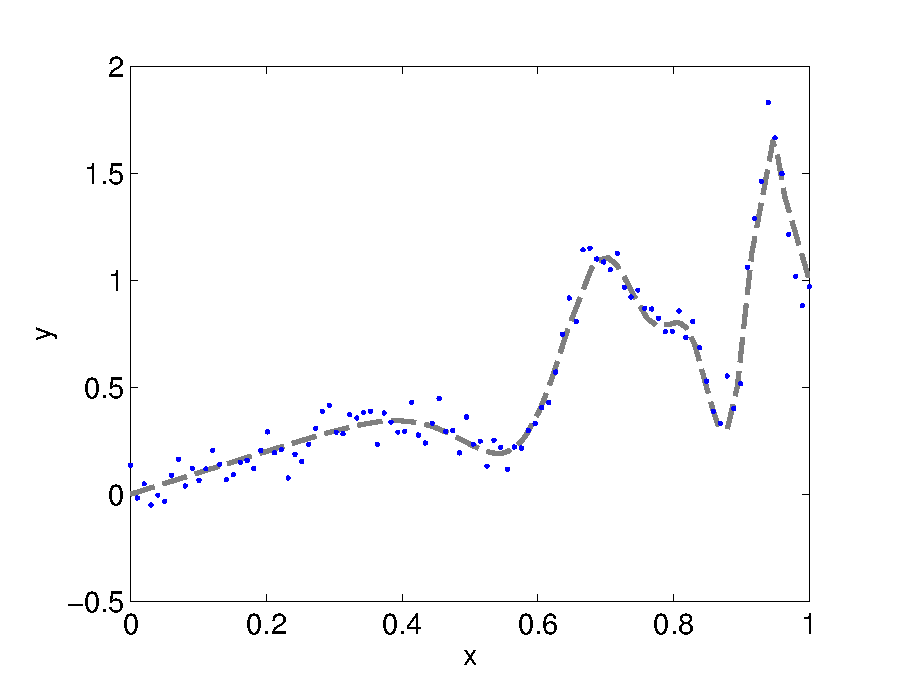
\includegraphics[width=.45\textwidth]{Figures/LLR-nonlinfunction}
	\label{fig:LLR-nonlinfunction_dataset}
	}\\
	\subfigure[\ac{LLR} estimate of the nonlinear function]{
	\includegraphics[width=.45\textwidth]{Figures/LLR-nonlinfunction_globalk}
	\label{fig:LLR-nonlinfunction_estimate}
	}\\
	\subfigure[Prediction interval compared to the estimation error]{
	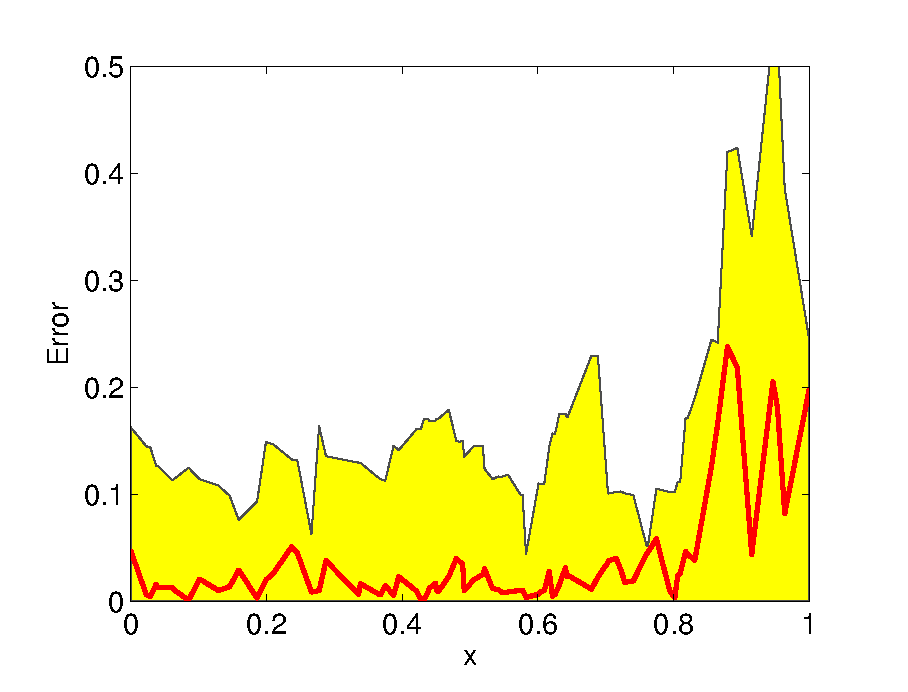
\includegraphics[width=.45\textwidth]{Figures/LLR-nonlinfunction_predint}
	\label{fig:LLR-nonlinfunction_predint}
	}
	\caption[\acs{LLR} estimate of a nonlinear function]{\ac{LLR} estimate of a 1-dimensional nonlinear function. \subref{fig:LLR-nonlinfunction_dataset} shows 100 noisy samples (dots) obtained from the nonlinear function \eqnref{eqn:LLR-nonlinear test function} (dashed line). \subref{fig:LLR-nonlinfunction_estimate} shows the resulting \ac{LLR} estimate (solid line) of the nonlinear function (dashed line) using $K=4$ with prediction intervals (shaded area) estimated at 100 query points. \subref{fig:LLR-nonlinfunction_predint} shows the estimation error $\left| \hat{y} - y \right|$ (solid red line) compared to the size of the prediction interval (shaded area).}
	\label{fig:LLR-nonlinfunction}
\end{figure}


\subsubsection{Outlier detection}
To test if we can use the methods of Section \ref{sec:LLR-outlierdetection} to identify faulty data, we replaced four samples of the original dataset of \figref{fig:LLR-nonlinfunction_dataset} by faulty data. \figref{fig:LLR-outlierdetection_without} shows the result that the outliers have on the estimation of the target function. We notice that the prediction is severely effected by the presence of the outliers. This is in turn represented by the prediction intervals, which are very large for the estimates that use the outliers.
 
\figref{fig:LLR-outlierdetection_with} shows the result when outlier detection is used. The data points that are identified as outliers are indicated by circles. When outliers were detected the \ac{LLR} estimate was computed again, neglecting the outlier(s). The added outliers are identified correctly. The result is clearly visible by the prediction intervals that are much smaller when the outliers are neglected. Also the \ac{LLR} estimate $\hat{y}$ becomes better when the outliers are neglected.

We notice that not only the added outliers are detected, but also the sample at $x = 0.72$ is identified as outlier. This is caused by the fact that the noisy data samples around this point are almost linear. This causes the identified linear model to match all points very accurately except for one point, which is therefore identified as outlier.

In our approach, we simply neglected outliers that were detected. An other approach could be to remove detected outliers from the memory. We do not opt for this approach because a sample that appears to be an outlier for a certain query point at one moment in time, could prove to be an usable sample for a different query point or at a later stage when more samples have been added to the memory. In general, we do not encourage removing or changing memory data. 
 
\begin{figure}[htbp]
	\centering
	\subfigure[Without outlier detection]{
	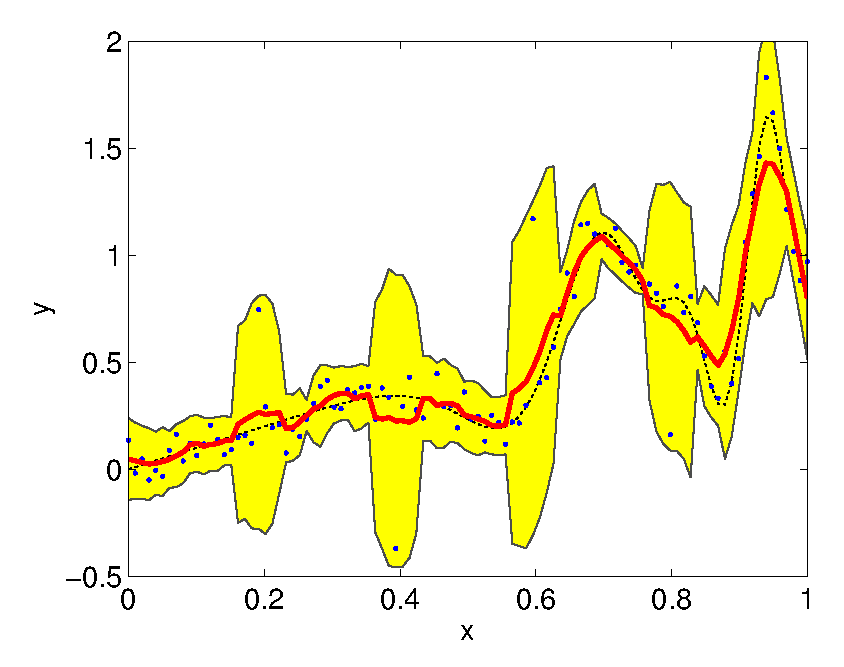
\includegraphics[width=.45\textwidth]{Figures/LLR-outlierdetection_without}
	\label{fig:LLR-outlierdetection_without}
	} 
	\subfigure[With outlier detection]{
	\includegraphics[width=.45\textwidth]{Figures/LLR-outlierdetection_with}
	\label{fig:LLR-outlierdetection_with}
	}
	\caption[Outlier detection in \ac{LLR}]{\ac{LLR} estimate with $K=4$ (solid line) of a nonlinear function (dashed line) with outliers added at $x=0.2,0.4,0.6,0.8$. \subref{fig:LLR-outlierdetection_without} shows the resulting estimate when the outliers are used in the estimation. \subref{fig:LLR-outlierdetection_with} shows the result when outliers are detected and neglected in the estimation. Data points that are identified as outliers are indicated by circles.}
	\label{fig:LLR-outlierdetection}
\end{figure}



\subsubsection{Optimizing the number of neighbors}\label{sec:LLR-optimal number of neighbors}
One of the attractive properties of \ac{LLR} is that the method has only got one parameter to tune: the number of nearest neighbors $K$ used in estimating the linear model. The optimal number of neighbors leads to the best estimation of the output (i.e., the smallest estimation error). The optimal number can vary throughout the state-space and depends locally on a number of factors:
\begin{itemize}
	\item Linearity of the function (highly nonlinear, smaller $K$)
	\item Sample density (more samples, higher $K$)
	\item Amount of noise (more noise, higher $K$)
\end{itemize}
Because these factors can vary over the state-space, the optimal number of nearest neighbors can also vary over the state-space. \figref{fig:LLR-optimal_K_schematic} schematically shows the estimation error as a function of $K$ for three different target functions:
\begin{enumerate}
	\item Linear function with noise
	\item Nonlinear function without noise
	\item Nonlinear function with noise
\end{enumerate}
In the first case (\figref{fig:LLR-optimal_K_schematic_a}), the number of neighbors should be high as possible to cancel the effect of noise. In fact, for white noise and $K\rightarrow \infty$ the \ac{LLR} estimate $\hat{y}(x_q)$ is an unbiased estimator of $y(x_q)$.

In the second case (\figref{fig:LLR-optimal_K_schematic_b}), the optimal choice is to simply take the output of the nearest neighbor as the estimated output. Including more neighbors will introduce a bias, since the target function is locally nonlinear.

The third case is the most interesting since this situation will generally be encountered in practice. Starting from $K=1$, increasing the number of nearest neighbors will reduce the estimation error, because the effect of noise is reduced. Further increasing $K$, will increase the error as the nonlinearity results in a biased estimate. So an optimal value for $K$ exists for which the estimation error is smallest.

Determining the optimal value for $K$ can be problematic, since no analytical expression to determine the optimal value for $K$ exists. Furthermore, even if we have a measure for the estimation error for a certain value of $K$, we do not have a method to determine whether this error is due to noisy samples or due to local nonlinearity of the target function. In the first case $K$ has to be increased, while in the second case it has to be decreased. In the next paragraph we will describe how the prediction interval could be used to tune the number of nearest neighbors.

\begin{figure}[htbp]
\centering
\subfigure[Linear target function with noise]{
\includegraphics[width=.3\textwidth]{img/Koptimal_schematic_a}
\label{fig:LLR-optimal_K_schematic_a}
}
\subfigure[Nonlinear target function without noise]{
\includegraphics[width=.3\textwidth]{img/Koptimal_schematic_b}
\label{fig:LLR-optimal_K_schematic_b}
}
\subfigure[Nonlinear target function with noise]{
\includegraphics[width=.3\textwidth]{img/Koptimal_schematic_c}
\label{fig:LLR-optimal_K_schematic_c}
}
	\caption[Optimal number of neighbors for three different target functions]{Optimal number of neighbors for three different cases. \subref{fig:LLR-optimal_K_schematic_a} linear target function with added noise, \subref{fig:LLR-optimal_K_schematic_b} nonlinear target function without noise and \subref{fig:LLR-optimal_K_schematic_c} nonlinear target function with added noise. The top figures show a typical distribution of data points and the resulting linear regression. The bottom figures show schematically the absolute value of the estimation error of the real output and the estimated output as a function of the number of neighbors $K$.}
	\label{fig:LLR-optimal_K_schematic}
\end{figure}
	

\paragraph{Globally optimal $K$}
The general approach to tuning the value of $K$ is using the globally optimal value. A global optimum means a single fixed $K$ value that leads to the best estimation error on average. In practice, this means computing a model for several values of $K$ for a set of query points. The value that leads to the smallest total residual value will be chosen as globally optimal. This approach will typically lead to a model that is too general in fast dynamics regions and too noise sensitive in slow dynamics regions.

\figref{fig:LLR-K_varying} shows the RMS error of the estimation of the dataset of \figref{fig:LLR-nonlinfunction_dataset} for a range of different $K$ values. Since the target function is noisy and nonlinear, we expect the behavior as depicted in \figref{fig:LLR-optimal_K_schematic_c}. The expected behavior (first a decrease in error, then an increase) is indeed visible. Based on this figure, we select the globally optimal value $K=4$. 
%\begin{figure}[htbp]
%	\centering
%%		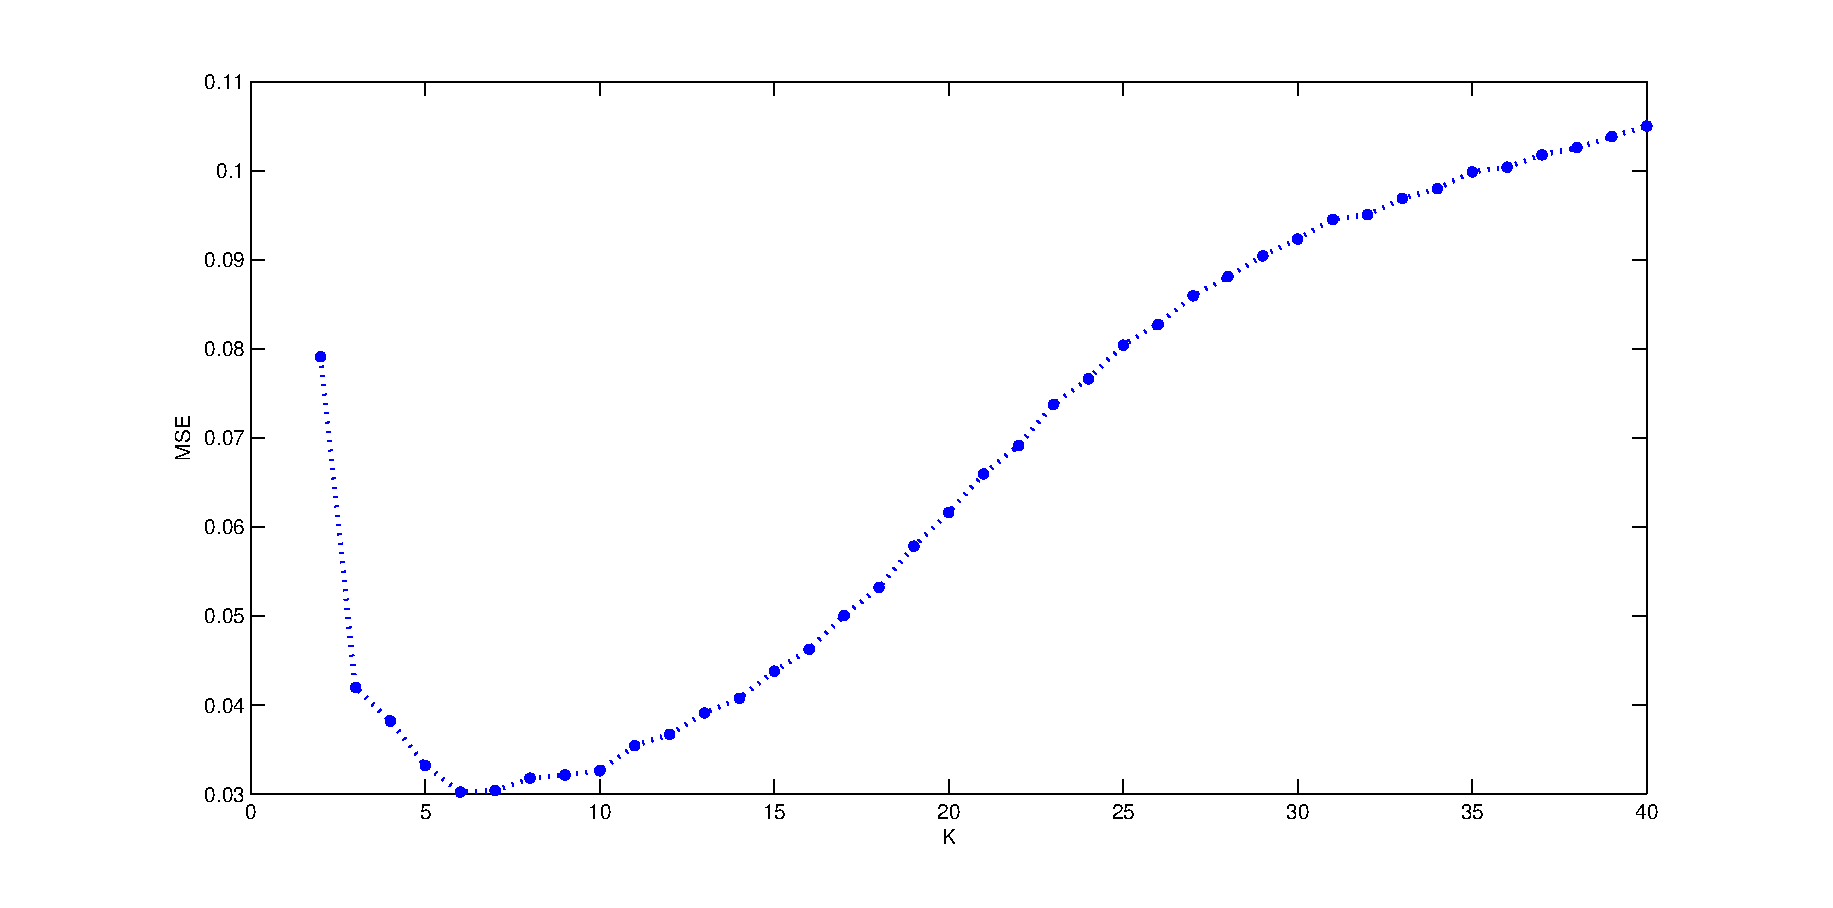
\includegraphics[width=.5\textwidth]{Figures/k_varying}
%		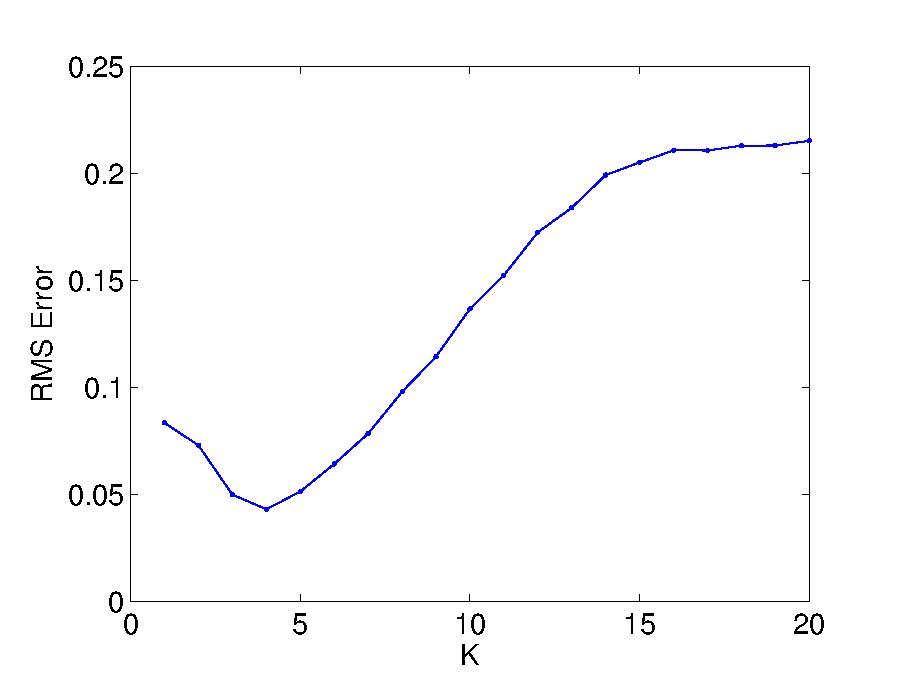
\includegraphics[width=.5\textwidth]{Figures/LLR-nonlinfunction_var_K}
%	\caption[Estimation error for a range of $K$ values]{RMS estimation error for a range of different $K$ values for the nonlinear target function.}
%	\label{fig:LLR-K_varying}
%\end{figure}

\begin{figure}[htbp]
	\centering
	\subfigure[Global optimum: $K=4$]{
	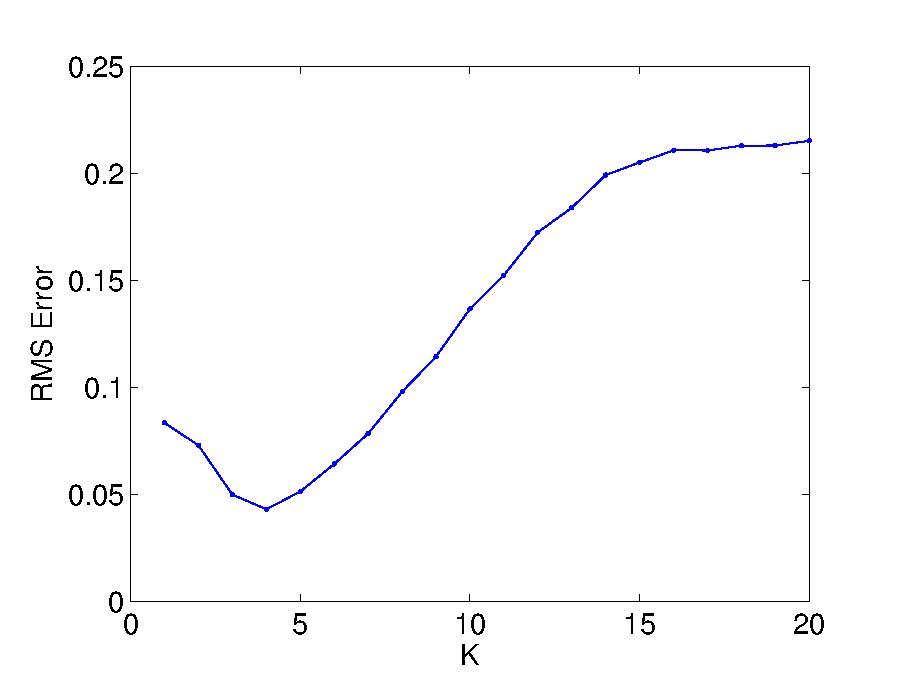
\includegraphics[width=.45\textwidth]{Figures/LLR-nonlinfunction_var_K}
	\label{fig:LLR-K_varying}
	} 
	\subfigure[Locally optimal $K$]{
	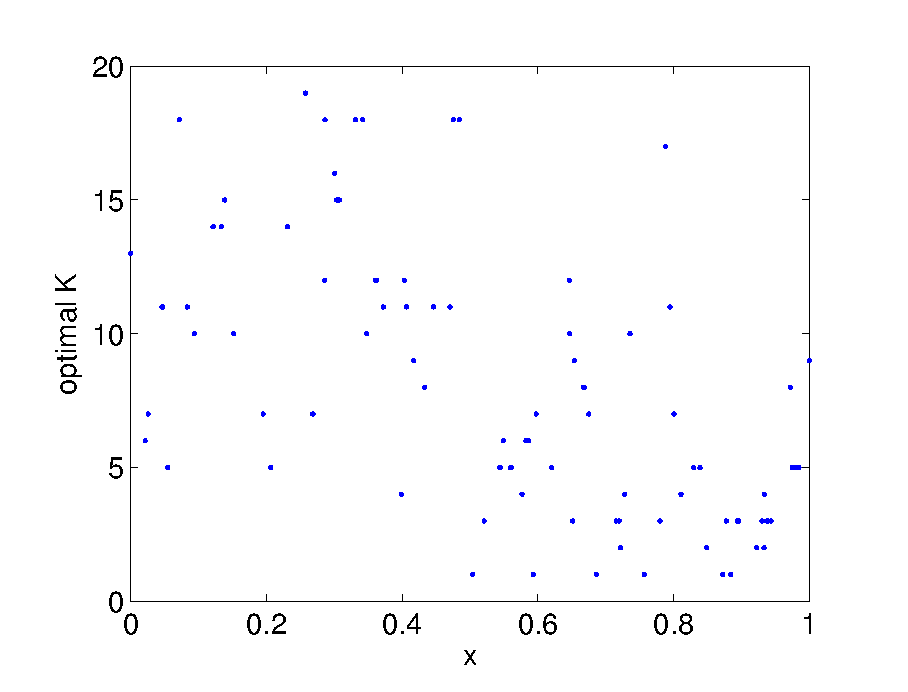
\includegraphics[width=.45\textwidth]{Figures/LLR-nonlinfunction_optimal_K}
	\label{fig:LLR-K_optimal}
	}
	\caption[Global versus local optimal $K$ value]{Comparison between global and local optimal $K$ values for the nonlinear target function \eqnref{eqn:LLR-nonlinear test function}. \subref{fig:LLR-K_varying} shows the \ac{RMS} error of the estimation for a range of different $K$ values. \subref{fig:LLR-K_optimal} shows the locally optimal value of $K$ for a range of $x$ values.}
	\label{fig:LLR-nonlinfunction_K}
\end{figure}

\paragraph{Locally optimal $K$}
A more advanced method of selecting $K$ is choosing a specific value for every query point. Using different values for every query point could lead to a better estimation quality on average. Unfortunately, an analytical formula for finding the optimal value does not exist, since the effect of an single unknown sample on the estimation quality is not known\footnote{Incremental linear regression methods that solve a least squares problem by adding samples one-by-one do exist. However, they do not give an analytical expression for the influence of a single sample on the output or the prediction accuracy.}. Therefore, the locally optimal value has to be found by computing the model for a set of $K$ values and selecting the one that is best according to some quality measure. Notice that this quality measure may only depend on the memory samples and not on the actual output, since this may be unknown. A possible quality measure could be the prediction interval discussed in Section \ref{sec:LLR-prediction interval}. We select the $K$ value that leads to the smallest prediction interval as optimal.

\figref{fig:LLR-K_optimal} shows the locally optimal value for $K$ for the nonlinear test function \eqnref{eqn:LLR-nonlinear test function}. It is clear that the optimal value varies heavily over the domain of the function. On closer inspection, we notice that the optimal value is in general smaller for larger $x$-values. This is due to the faster dynamics of the test function for these values of $x$. For smaller $x$-values the optimal value is larger due to the slower dynamics.
%\begin{figure}[htbp]
%	\centering
%		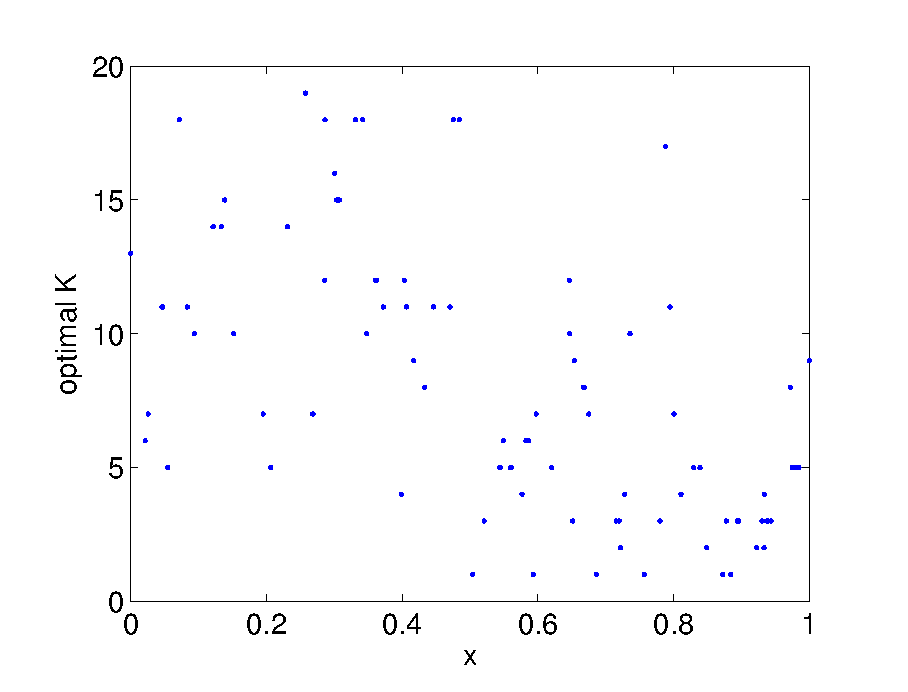
\includegraphics[width=.5\textwidth]{Figures/LLR-nonlinfunction_optimal_K}
%	\caption[Optimal $K$ value]{Locally optimal value of $K$ for the nonlinear test function \eqnref{eqn:\ac{LLR}-nonlinear test function}.}
%	\label{fig:LLR-K_optimal}
%\end{figure}

The difference between a locally and globally optimal value of $K$ is shown in \figref{fig:LLR-nonlinfunction_K_local_global}. The global $K$ value is set to $K=4$. We notice that the prediction interval is smaller using a locally optimal $K$. This is as expected, since this is the quantity we minimized in selecting $K$. However, if we look at the estimated values, the results vary. In high frequency regions (near $x=0.85$ and $x=0.95$) we notice that the estimate improves when a locally optimized $K$ value is used. In low frequency regions (near $x=0.05$ and $x=0.45$ for example), the estimation becomes worse. This is due to the fact that a linear model is fitted to a small number of noisy samples. 

\begin{figure}[htbp]
\centering
\subfigure[Globally fixed $K=4$]{
\includegraphics[width=.45\textwidth]{Figures/LLR-nonlinfunction_globalk}
\label{fig:LLR-nonlinfunction_globalk}
} 
\subfigure[Locally optimal $K$]{
\includegraphics[width=.45\textwidth]{Figures/LLR-nonlinfunction_localk}
\label{fig:LLR-nonlinfunction_localk}
}
\caption[\ac{LLR} estimate of a nonlinear function]{\ac{LLR} estimate (solid red line) of a nonlinear function (dashed line) with prediction intervals (shaded area). \subref{fig:LLR-nonlinfunction_globalk} shows the resulting estimate for a globally optimal (fixed) value of $K$. \subref{fig:LLR-nonlinfunction_localk} shows the result for a locally optimal (varying) value of $K$.}
\label{fig:LLR-nonlinfunction_K_local_global}
\end{figure}

Whether or not a locally optimized $K$-value leads to better estimations than a globally optimized value will depend on the situation. In very noisy applications, using the prediction interval to determine a locally optimal value might lead to bad estimates. A globally optimal $K$ value is probably a good choice is most situations. In the remaining experiments, we selected a globally optimal $K$ value in a way very similar to the approach described in this section. 





\subsection{Two-link manipulator}\label{sec:LLR-two link manipulator}
In this section we will use \ac{LLR} to model state-transitions of a realistic setup. We consider a two-link manipulator system (see \figref{fig:LLR-twolinkmanipulator}). It was chosen because of its relative simplicity and because of its connection with a humanoid robot setup. The manipulator resembles one leg of a humanoid robot, actuated at the knee and hip joints. If this setup leads to good results, it gives confidence that \ac{LLR} might also be used to model a real humanoid robot setup.
\begin{figure}[htbp]
	\centering
		\includegraphics[width=.1\textwidth]{img/twolinkmanipulator}
	\caption[Two-link manipulator setup]{Two-link manipulator setup.}
	\label{fig:LLR-twolinkmanipulator}
\end{figure}

%\paragraph{System}\label{sec:LLR-two link manipulator system}
The two-link manipulator consists of two actuated joints, connected with rigid arms. The system is fixed at one of the joints. The setup is placed vertically. The system has a 4 state-variables: the two angles $\bm{\theta} = \begin{bmatrix} \theta_1 & \theta_2 \end{bmatrix}^T$ and two angular velocities $\bm{\omega} = \begin{bmatrix}\omega_1 & \omega_2 \end{bmatrix}^T$ of both joints. The full state-vector is $\mathbf{x} =  \begin{bmatrix} \bm{\theta} & \bm{\omega} \end{bmatrix}^T$. The input of the system are the output voltages to the motors: \lsymb{$\mathbf{u}$}{Input vector}$ = \begin{bmatrix} u_1 & u_2 \end{bmatrix}^T$. The voltages are limited to $\begin{bmatrix} 1.5 & 1 \end{bmatrix}^T$. The angles are limited to $[-\pi \quad \pi]$. The system is controlled at discrete time intervals $t$, with sampling time $T_s = 0.05$~s. The equations of motion are nonlinear and are given by:
$$
	M(\bm{\theta})\dot{\bm{\omega}}+ C(\bm{\theta}, \bm{\omega}) \bm{\omega} + G(\bm{\theta}) = \mathbf{u}
$$
\begin{eqnarray}
	M(\bm{\theta}) &=& \begin{bmatrix}
	P_1 + P_2 + 2P_3 \cos{\theta_2} & P_2 + P_3 \cos{\theta_2} \\
	P_2 + P_3 \cos{\theta_2} & P_2 \end{bmatrix} \nonumber
	\\
	C(\bm{\theta}, \bm{\omega}) &=& 
	\begin{bmatrix} b_1 - P_3 \omega_2 \sin{\theta_2} & P_3(\omega_1+\omega_2) \sin{\theta_2} \\
	P_3 \omega_2 \sin{\theta_2} & b_2 \end{bmatrix} \nonumber
	\\
	G(\bm{\theta}) &=& \begin{bmatrix} -g_1 \sin{\theta_1}-g_2 \sin{(\theta_1 + \theta_2)} \\
	-g_2 \sin{(\theta_1+\theta_2)} \end{bmatrix} \nonumber
\end{eqnarray}
The abbreviations are defined as follows:
\begin{eqnarray}
	P_1 =& m_1c_1^2 + m_2l_1^2 + I_1 \nonumber \\
	P_2 =& m_2c_2^2 + I_2 \nonumber \\
	P_3 =& m_2l_1c_2 \nonumber \\
	g_1 =& (m_1c_1 + m_2l_1)g \nonumber \\
	g_2 =& m_2c_2g \nonumber
\end{eqnarray}
The parameters of the system and their physical meanings can be found in \tabref{tab:LLR-two link manipulator parameters}.
\begin{table}[htbp]
	\centering
	\caption[Two-link manipulator: Parameter values]{Physical parameters of the two-link manipulator}
		\begin{tabular}{ll}
			Symbol & Parameter \\ \hline
			$g = 9.81 \textrm{ m/s}^2$ & gravitational acceleration \\
			$l_1 = 0.4$ m & length of first link \\
			$l_2 = 0.4$ m & length of second link \\
			$m_1 = 1.25$ kg & mass of first link \\ 
			$m_2 = 0.8$ kg & mass of second link \\
			$I_1 = 0.07 \textrm{ kgm}^2$ & inertia of first link \\ 
			$I_2 = 0.04 \textrm{ kgm}^2$ & inertia of second link \\ 
			$c_1 = 0.2$ m & center of mass of first link \\
			$c_2 = 0.2$ m & center of mass of second link \\
			$b_1 = 0.08$ kg/s & damping in first joint \\
			$b_2 = 0.02$ kg/s & damping in second joint
		\end{tabular}
	\label{tab:LLR-two link manipulator parameters}
\end{table}

%\subsubsection{Experimental setup}\label{sec:LLR-two link manipulator experimental setup}
The model was implemented as a simulation in Matlab. A white noise signal with $\sigma^2 = 0.01$ was added to each output. The following input-output relation was estimated:
$$
	\hat{\mathbf{x}}_{t+1} = \begin{bmatrix} \mathbf{x}_t \\ \mathbf{u}_t \\ 1 \end{bmatrix}^T \hat{\bm{\beta}}
$$
with $\hat{\bm{\beta}}$ the local linear model. A dataset was generated by applying a random input signal to the system and observing the resulting state-transitions for 250 seconds (5000 samples). The memory was filled with state-transition samples: $(\mathbf{x}_t,\mathbf{u}_t,\mathbf{x}_{t+1})$. The number of nearest neighbors used in the experiments was fixed to $K=10$.

The two-link manipulator setup was used to investigate some of the properties of the \ac{LLR} method in a setting that resembles a real learning experiment. We are mainly interested in the ability of \ac{LLR} to model state-transitions and the influence of the memory size on the estimation accuracy. Furthermore, we are interested if fitting a linear model to a set of nearest neighbors improves the estimation compared to more simpler memory-based methods. We can summarize these questions as follows:
\begin{enumerate}
	\item Can \ac{LLR} be used to model state-transitions?
	\item How does the memory size influence the estimation accuracy?
	\item Is \ac{LLR} an improvement over other memory-based methods?
\end{enumerate}



%\subsubsection{Results}\label{sec:LLR-two link manipulator results}
\subsubsection{Estimating state-transitions}\label{sec:LLR-2link_statetransitions}
\begin{figure}[htbp]
	\centering
	\subfigure[Memory size: $N=200$ (10 s)]{
		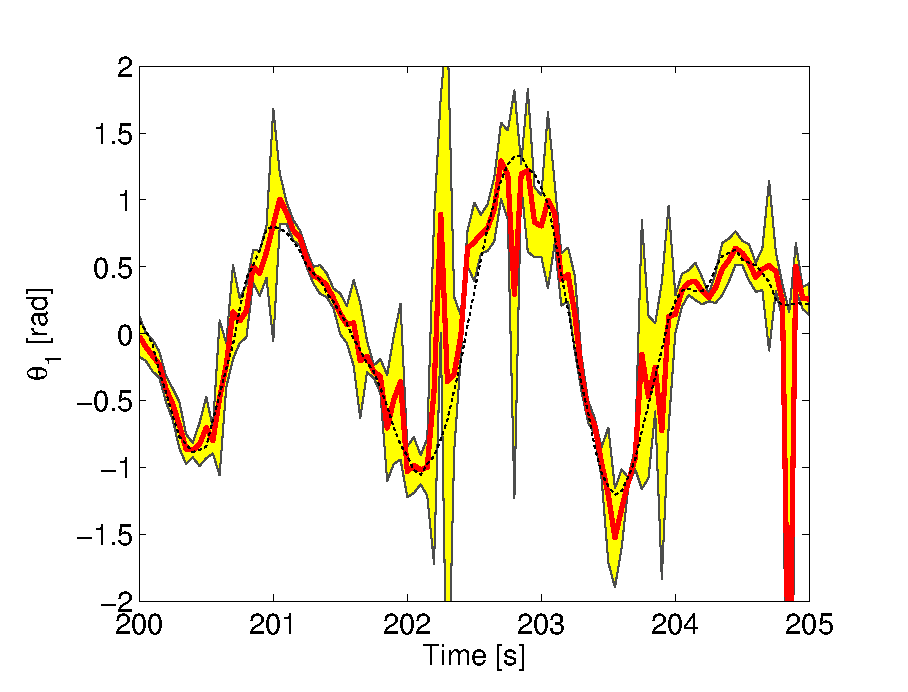
\includegraphics[width=.4\textwidth]{Figures/LLR-robotarm_theta1}
		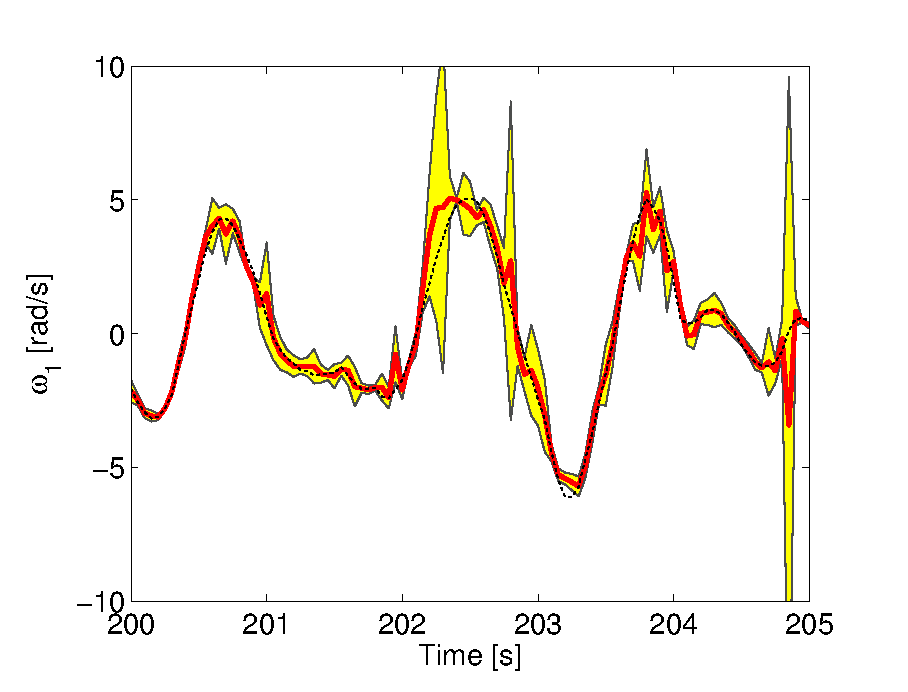
\includegraphics[width=.4\textwidth]{Figures/LLR-robotarm_omega1}
		\label{fig:LLR-RobotarmIncr_N1}
	}\\
	\subfigure[Memory size: $N=4000$ (200 s)]{
		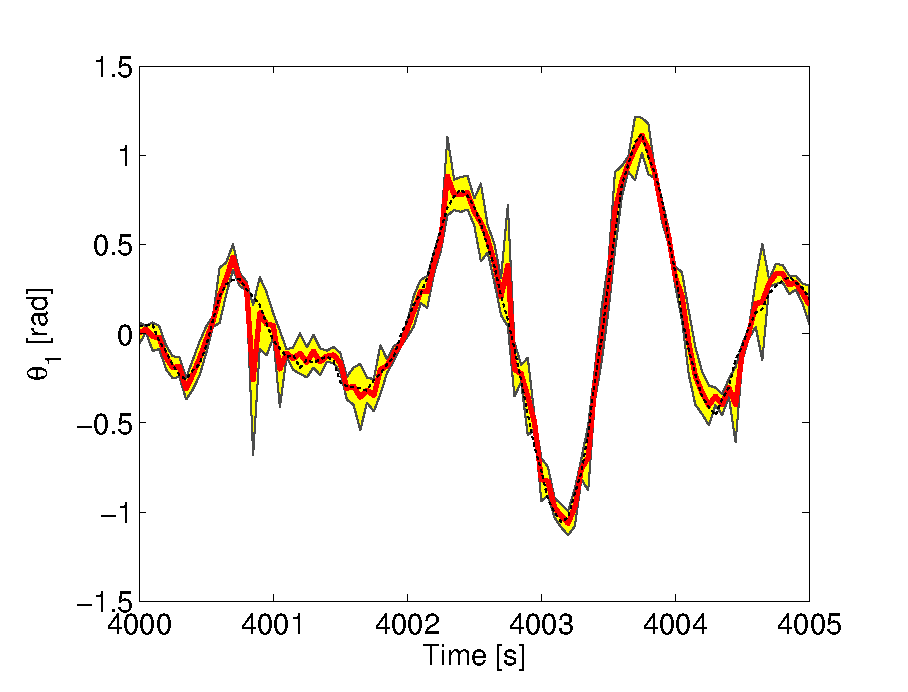
\includegraphics[width=.4\textwidth]{Figures/LLR-robotarm_theta2}
		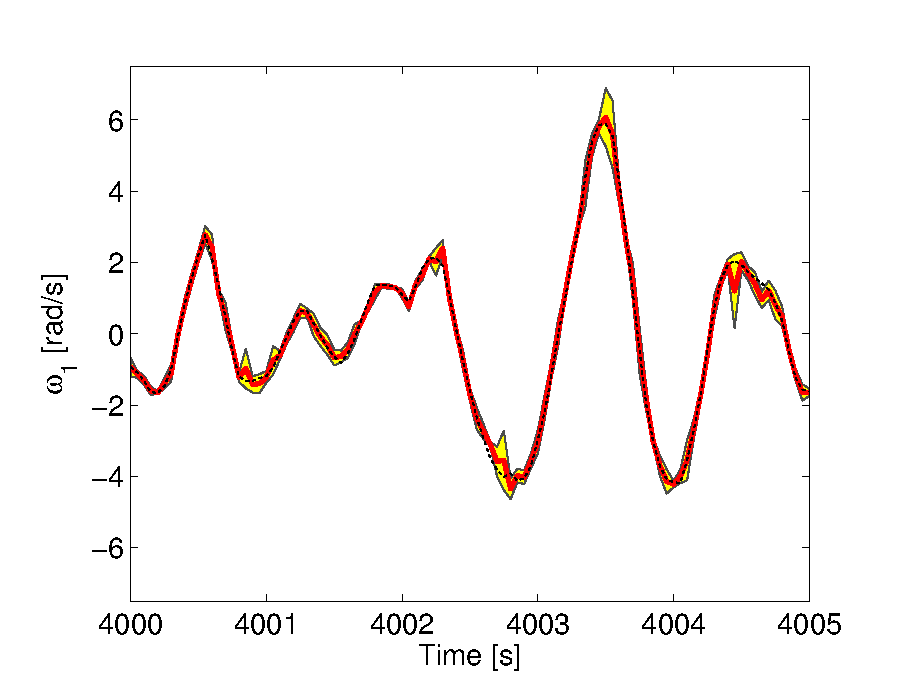
\includegraphics[width=.4\textwidth]{Figures/LLR-robotarm_omega2}
		\label{fig:LLR-RobotarmIncr_N2}
	}
	\caption[\ac{LLR} estimate of the two-link manipulator]{\ac{LLR} estimate of state-transitions for the two-link manipulator for increasing memory size using $K=10$. The figures show the improvement of the \ac{LLR} estimate for $\theta_1$ (left figures) and $\omega_1$ (right figures). \subref{fig:LLR-RobotarmIncr_N1} is the estimate using a memory of size $N=200$ (10 seconds), \subref{fig:LLR-RobotarmIncr_N2} the estimate for $N=4000$ (200 seconds). The figures show the \ac{LLR} estimate (red solid line), the measured value (black dashed line) and the prediction intervals (shades areas).}
	\label{fig:LLR-RobotarmIncr}
\end{figure}
In a typical real-world learning experiment, the size of the memory available to the model increases during the experiment. We mimic this situation by increasing the size of the memory available to the \ac{LLR} algorithm. At every time step, the model uses the memory samples observed up until that moment. These memory samples are used to estimate the transition from the current state to the next. We expect that the estimations become better with increasing memory size. \figref{fig:LLR-RobotarmIncr} shows the estimated state-transitions at two moments in the experiment for the angle $\theta_1$ and angular velocity $\omega_1$ of the first link. The state-variables of the second link show the same behavior and are therefore not shown. 

The first observation that has to be made, is the fact that \ac{LLR} is indeed able to model state-transitions. Using state-action pairs as input, the resulting next state can be estimated as output. Especially with a large memory (\figref{fig:LLR-RobotarmIncr_N2}), the estimated state-transitions closely match the real state-transitions. It appears that the prediction intervals can be used as a measure for the estimation accuracy. We notice that state-transitions that are estimated inaccurately, also have a relatively large prediction interval. Especially with a large memory, the prediction intervals are small compared to the amplitude of the variables. 

The improvement of the estimate with increasing memory size, is also visualized in \figref{fig:LLR-robotarm_RMSE_compare}. The figure shows the RMS error of the estimated state-transitions. The estimation improves with the first 1000 samples and is more or less equal thereafter.
\begin{figure}[htbp]
	\centering
		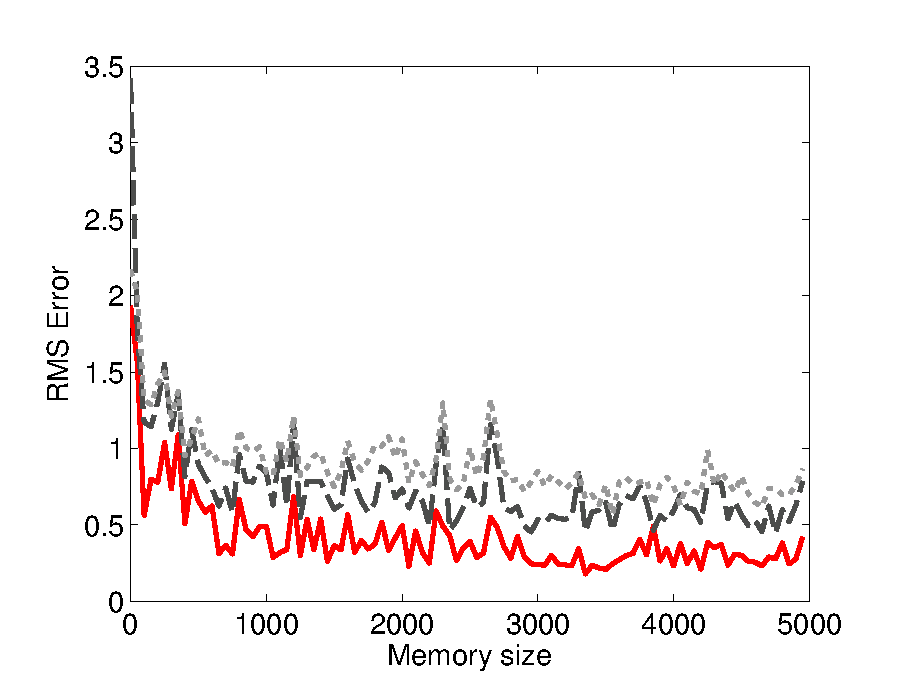
\includegraphics[width=0.5\textwidth]{Figures/LLR-robotarm_RMSE_compare}
		\caption[Estimation error for the two-link manipulator for increasing memory size]{\ac{RMS} estimation error for increasing memory size using different methods to estimate the two-link manipulator. The figure compares the nearest neighbor estimate ($K=1$, dotted gray line), the $K$ nearest neighbors average ($K=10$, dashed gray line) and the \ac{LLR} estimate ($K=10$, solid red line).}
	\label{fig:LLR-robotarm_RMSE_compare}
\end{figure}


%\paragraph{Comparing model-based modeling methods} 
\subsubsection{Comparing memory-based modeling methods}\label{sec:LLR-2link_ModelBasedComparison}

\begin{figure}[htbp]
	\centering
		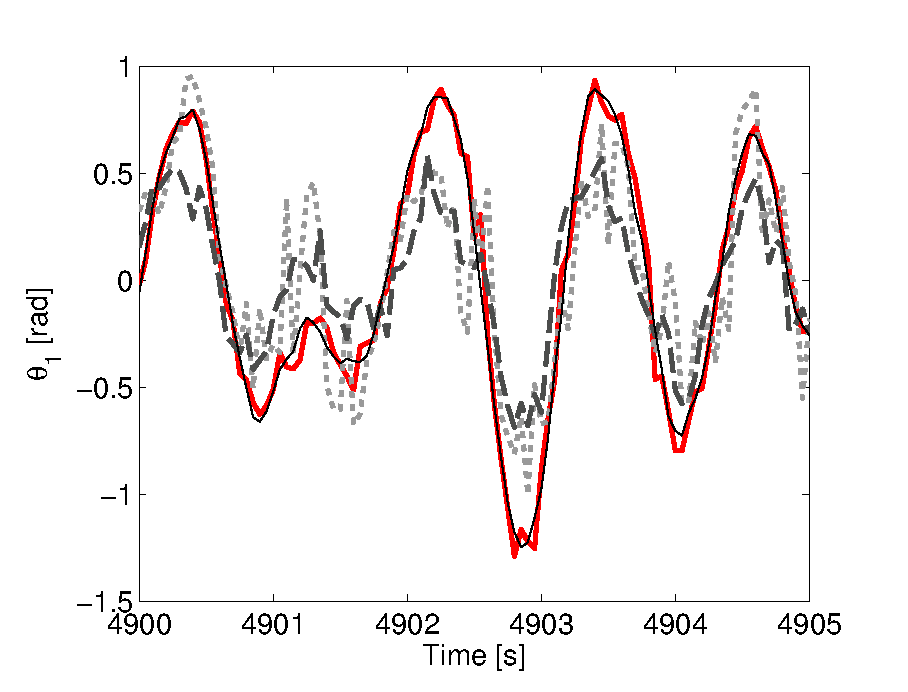
\includegraphics[width=0.5\textwidth]{Figures/LLR-robotarm_trajectory}
		\caption[Comparing three memory-based modeling methods]{Comparison of three memory-based modeling methods on the two-link manipulator using a large memory ($N=5000$). The figure shows the estimation of a trajectory (solid black line) using the nearest neighbor ($K=1$, dotted gray line), the $K$ nearest neighbors average ($K=10$, dashed gray line), and the \ac{LLR} estimate ($K=10$, solid red line).}
	\label{fig:LLR-robotarm_trajectory}
\end{figure}
We have introduced \ac{LLR} as a memory-based modeling method that fits a linear model to the set of nearest neighbors around the query input. Linear regression is a time consuming process, so the question rises whether fitting a linear model to the set of nearest neighbors is needed. Instead of estimating a model, we could also use the average output of the nearest neighbors as estimate (the $K$ nearest neighbors average). An even faster option is to simply use the output of the nearest neighbor ($K=1$) as an estimation for the output.
 
\figref{fig:LLR-robotarm_trajectory} compares these three memory-based methods by estimating a 5-second trajectory using a random input signal and a large memory ($N=5000$) to estimate state-transitions. We see that over the entire trajectory the \ac{LLR} method outperforms the other memory-based methods. It seems that the other methods give an estimate that is too conservative. \figref{fig:LLR-robotarm_RMSE_compare} confirms this by showing that the \ac{RMS} estimation error of \ac{LLR} is smaller than the other memory-based methods for all memory sizes. \figref{fig:LLR-robotarm_trajectory} shows that the difference in estimation quality is significant, so we conclude that fitting a linear model to the set of nearest neighbors leads to much better state-transition estimates. We argue that the improvement in estimation quality is worth the extra computational effort needed to estimate the linear model.








\subsection{Humanoid robot}\label{sec:LLR-robot leo}
In this section we use a two-legged humanoid robot called `Leo' as experimental setup. Leo is a humanoid robot developed at Delft University as a test platform to perform \ac{RL} experiments (\figref{fig:LLR-Leo}). It was designed to be able to walk autonomously in circles. It is connected via a boom construction to a central rotating pivot, so it can theoretically walk infinitely long in circles. It has an arm that makes it possible to stand up when fallen. The setup is highly complex and is usable for performing advanced reinforcement learning experiments. We use it as a setup to test the ability of \ac{LLR} to model complex, real-world systems.
\begin{figure}[htbp]
	\centering
		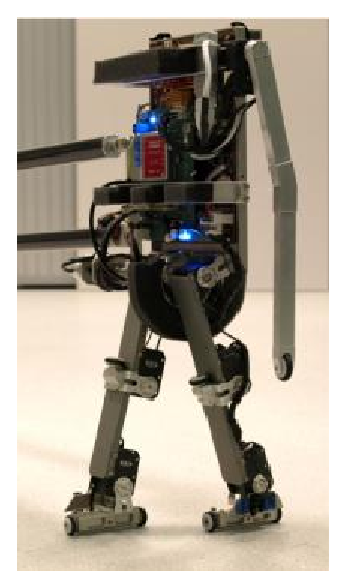
\includegraphics[width=.2\textwidth]{img/leo1}
	\caption[Humanoid robot setup]{Two-legged humanoid robot 'Leo'.}
	\label{fig:LLR-Leo}
\end{figure}
The robot is actuated at its angles, knees and hips. The motors also act as sensors that measure angle and angular velocity. Apart from the actuators, there are also sensors in the feet (that detect whether or not a foot touches the ground) and in the boom construction (measuring angle and angular velocity of the torso). In total, the robot has got 18 state-variables and 6 inputs. The states are concatenated in a $1\times 18$ row vector $\mathbf{x}$ and the actions in a $1\times 6$ row vector $\mathbf{u}$. The \ac{LLR} model $\hat{\bm{\beta}}$ estimates the state-transition from a state $\mathbf{x}_t$ to the next state $\mathbf{x}_{t+1}$ when actuated with action $\mathbf{u}_t$: 
$$
	\hat{\mathbf{x}}_{t+1} = \begin{bmatrix} \mathbf{x}_t \\ \mathbf{u}_t \\ 1 \end{bmatrix}^T \hat{\bm{\beta}}
$$

%\subsubsection{Experimental setup}\label{sec:LLR-robot leo experimental setup}
A large number of memory samples was gathered by letting Leo walk for about two minutes sampling at $150$~Hz using a pre-programmed controller. Although the walking motion looks to be the same in every step, closer inspection of the data reveals differences in every step (due to variations in the floor and other disturbances). The total dataset was split into two parts (both consisting of 8000 samples): one set for estimating the model and one for validating it. We used $K = 40$ for all Leo experiments. This value was determined empirically to give satisfactory results.

We have used \ac{LLR} to model this system to investigate its performance on modeling complex systems. The questions to be answered are:
\begin{enumerate}
	\item Can \ac{LLR} be used to model a complex, high-dimensional system?
	\item How large does the memory need to be for a reasonable estimation?
\end{enumerate}


%\subsubsection{Results}\label{sec:LLR-robot leo results}

%\paragraph{Modeling with large memory}
\subsubsection{Modeling walking motion}\label{sec:LLR-Leo_FullMemory} 
To show that the \ac{LLR} method is able to accurately model a high-dimensional system, we estimated the state-transitions of the validation dataset. The \ac{LLR} estimates were determined using the estimation dataset ($N=8000$) as memory. \figref{fig:LLR-LeoFullMemStep} shows the response of the real system and its \ac{LLR} estimate of one stride (two steps). For clarity we do not show all 18 state-variables but only the torso, the left hip and left foot (the estimates of all 18 state-variables can be found in Appendix \ref{app:LeoWalking}). We show these three variables, since they represent the remaining state-variables very well. Furthermore, since all estimated steps in the dataset are estimated approximately equally good, we show only one stride. 

We notice that in all three cases the output is estimated very accurate. In fact, the measured states are barely visible due to the very close estimates of the \ac{LLR} model. Also the prediction intervals are small (especially for the torso and the left hip), which indicates that the estimates are based on sets of very linear data. Although all variables are estimated accurately, the torso angle is clearly estimated best and the foot contact worst. This is reflected by the prediction intervals, which are small for the torso and hip, but larger for the foot. The main reason for this, is that the foot sensor data is very noisy. This is also visible from inspection of the measured data. 


\begin{figure}[htbp]
\centering
\subfigure[Torso angle]{
\includegraphics[width=.3\textwidth]{Figures/LLR-LeoFullMemStep_Torso}
\label{fig:LLR-LeoFullMemStep_Torso}
}
\subfigure[Left hip angle]{
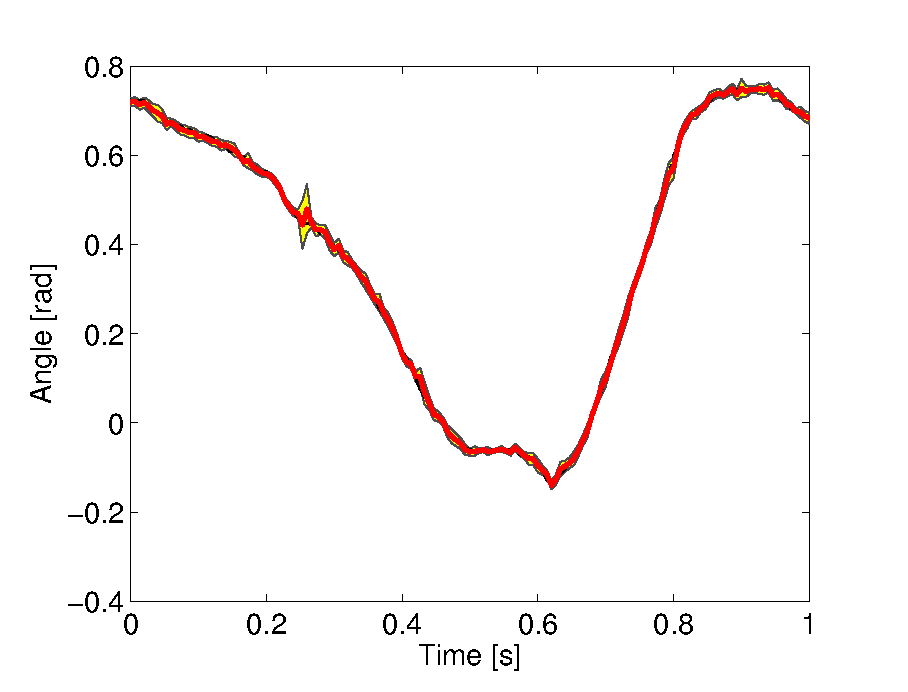
\includegraphics[width=.3\textwidth]{Figures/LLR-LeoFullMemStep_HipLeft}
\label{fig:LLR-LeoFullMemStep_HipLeft}
}
\subfigure[Left foot contact]{
\includegraphics[width=.3\textwidth]{Figures/LLR-LeoFullMemStep_Foot}
\label{fig:LLR-LeoFullMemStep_Foot}
} 
\caption[\ac{LLR} estimate of Leo walking]{\ac{LLR} estimate ($K=40$) of the walking motion of robot Leo using a memory consisting of 8000 samples. Three of the total of 18 state-variables are shown for one stride (two steps). \subref{fig:LLR-LeoFullMemStep_Torso} shows the angle of the torso, \subref{fig:LLR-LeoFullMemStep_HipLeft} shows the angle of the left hip, \subref{fig:LLR-LeoFullMemStep_Foot} the voltage of the left foot sensor. The figures show the \ac{LLR} estimate (solid red line), the measured output (dashed black line) and the prediction interval (shaded area).}
\label{fig:LLR-LeoFullMemStep}
\end{figure}

%\paragraph{Modeling with increasing memory} 
\subsubsection{Modeling using increasing memory}\label{sec:LLR-Leo_IncrMemory} 
In order to see the effect of the memory size on the estimation quality, we will again estimate the walking motion, but this time using a memory that increases in size. Starting with an empty memory, a new sample from the estimation dataset is added to the memory at every time step. This resembles a learning experiment which is started from no initial knowledge about the environment, but acquires one new state-transition at every time step.

\figref{fig:LLR-LeoIncrMemStep} shows the improvement of the \ac{LLR} estimate for state-variables torso angle, left hip angle and left foot contact. We show the \ac{LLR} estimates of the three variables for increasing memory size. The torso angle and left hip angle are estimated quite accurately, even from a very small number of memory samples. This is probably due to the similarity between different footsteps for these variables. On the other hand, the foot contact variable is estimated relatively badly, particularly for a small number of memory samples. This is visualized by the bad estimates and the large prediction intervals. As noted before, the bad estimate of the foot sensor is probably due to the noisy and therefore unpredictable behavior of this variable.
 
\figref{fig:LLR-LeoIncrMemError} shows the \ac{RMS} error of the estimation for an increasingly large memory. The estimation error variates during a step. In order to obtain a more smooth graph, we averaged the \ac{RMS} value over an estimated step (about $0.5$~s). So, the graph shows the average \ac{RMS} error of about 100 estimated steps. As expected, we see that the estimation error decreases with increasing memory size. The error decreases up to approximately $N = 2000$ and is more or less constant thereafter. This is approximately equal to 13 strides. So the \ac{LLR} method is able to estimate future steps accurately from 26 previously observed steps. Along with the RMS error of the estimation, we also plotted the \ac{RMS} value of the prediction interval. We notice that the prediction interval has a remarkably similar shape. Because the prediction interval can be considered as  a measure of linearity, this indicates that the size of the estimation error can be related to the nonlinearity of the memory samples. This is a direct consequence of the lack of appropriate nearest neighbors, which then leads to an inaccurate estimate of the state-transition for a particular state-action pair.

Although walking seems to be a motion that is the same in every step, in practice every single step is slightly different due to small disturbances such as ground level variations. This is reflected by sudden increases in the estimation error, for example around $N=4500$. Apparently this step was very different from the previously observed steps and the lack of appropriate nearest neighbors led to a \ac{LLR} estimate that is much worse than for previously estimated steps. This is confirmed by comparing the actual measurements of this step to other steps.

\begin{figure}[htbp]
\centering
\subfigure[Memory size: $N=150$ (2 steps)]{
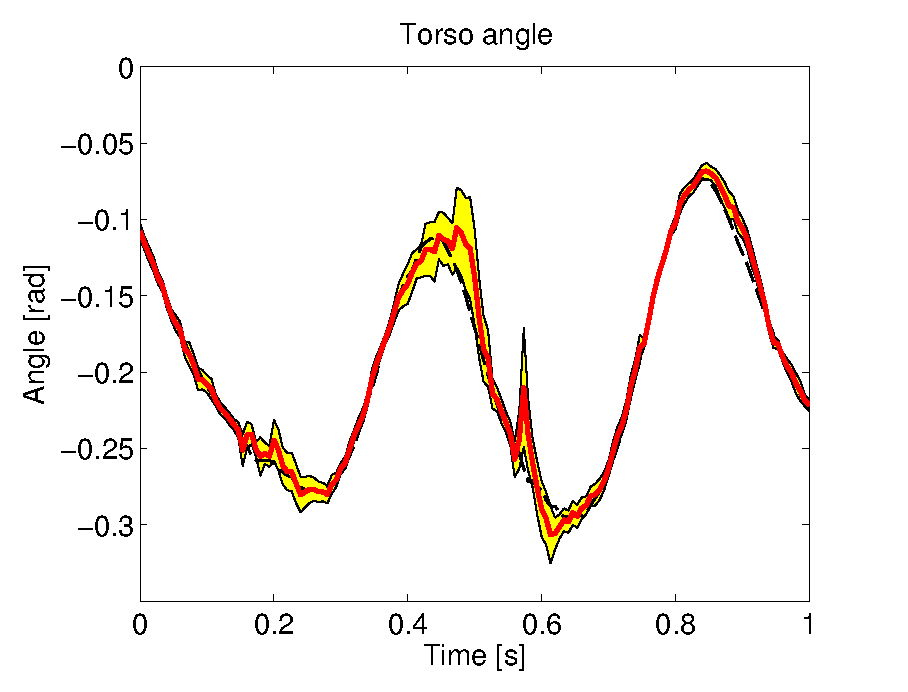
\includegraphics[width=.3\textwidth]{Figures/LLR-LeoIncrMemStep_Torso1}
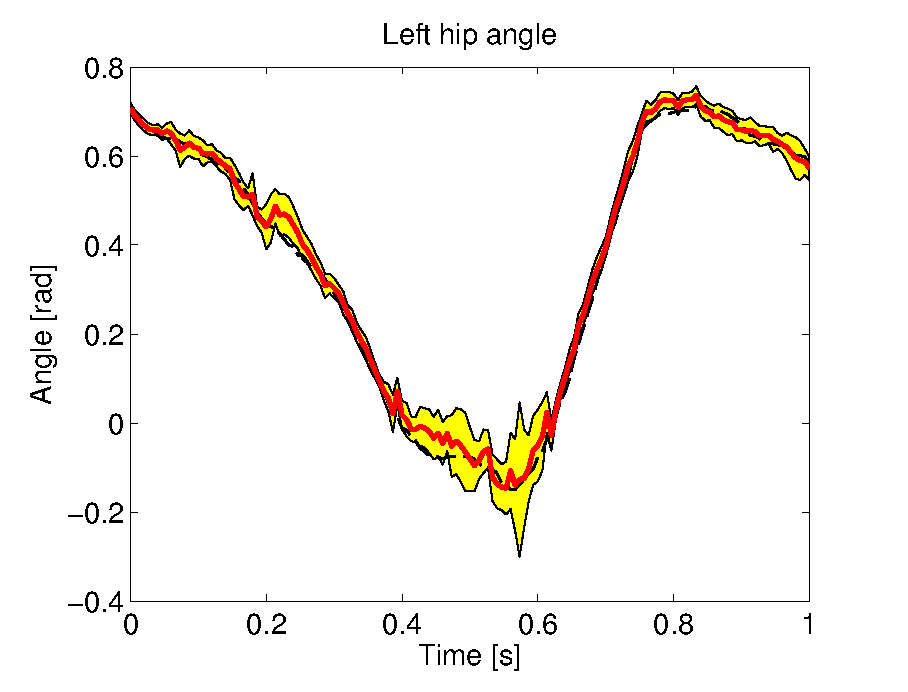
\includegraphics[width=.3\textwidth]{Figures/LLR-LeoIncrMemStep_HipLeft1}
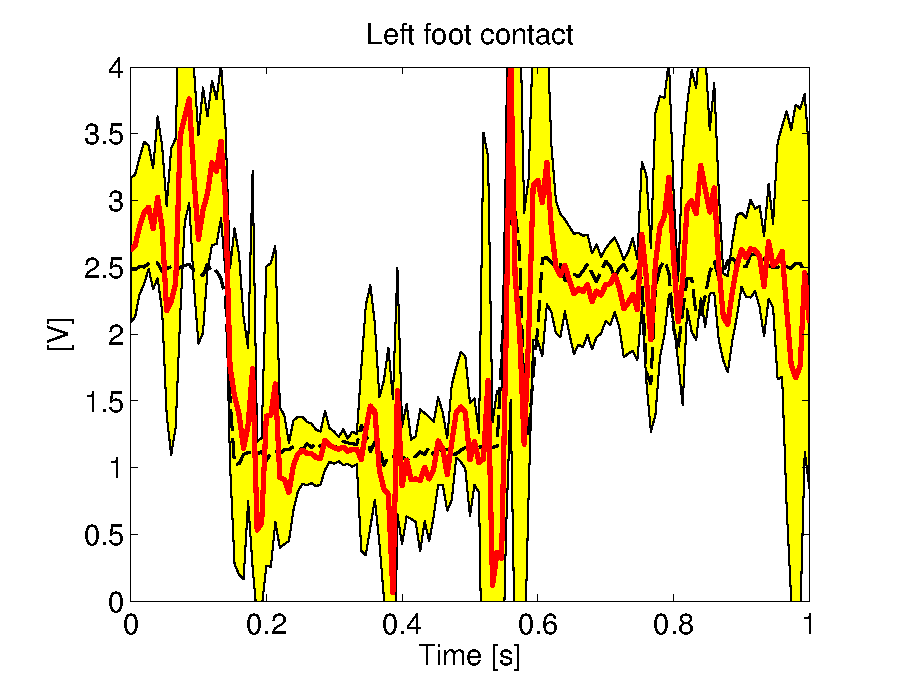
\includegraphics[width=.3\textwidth]{Figures/LLR-LeoIncrMemStep_Foot1}
\label{fig:LLR-LeoIncrMemStep_N1}
}\\
\subfigure[Memory size: $N=1000$ (14 steps)]{
\includegraphics[width=.3\textwidth]{Figures/LLR-LeoIncrMemStep_Torso2}
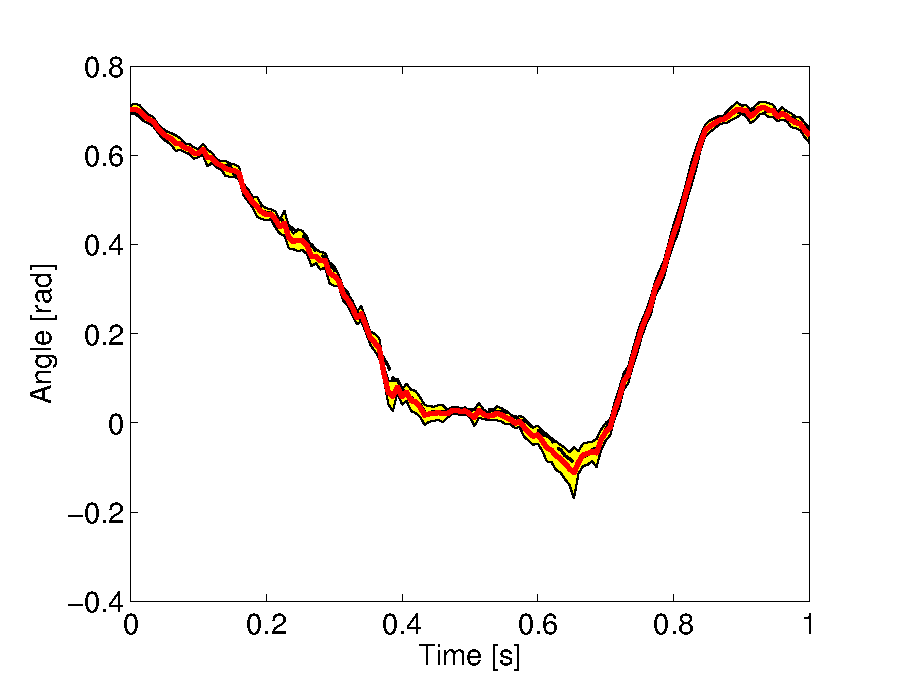
\includegraphics[width=.3\textwidth]{Figures/LLR-LeoIncrMemStep_HipLeft2}
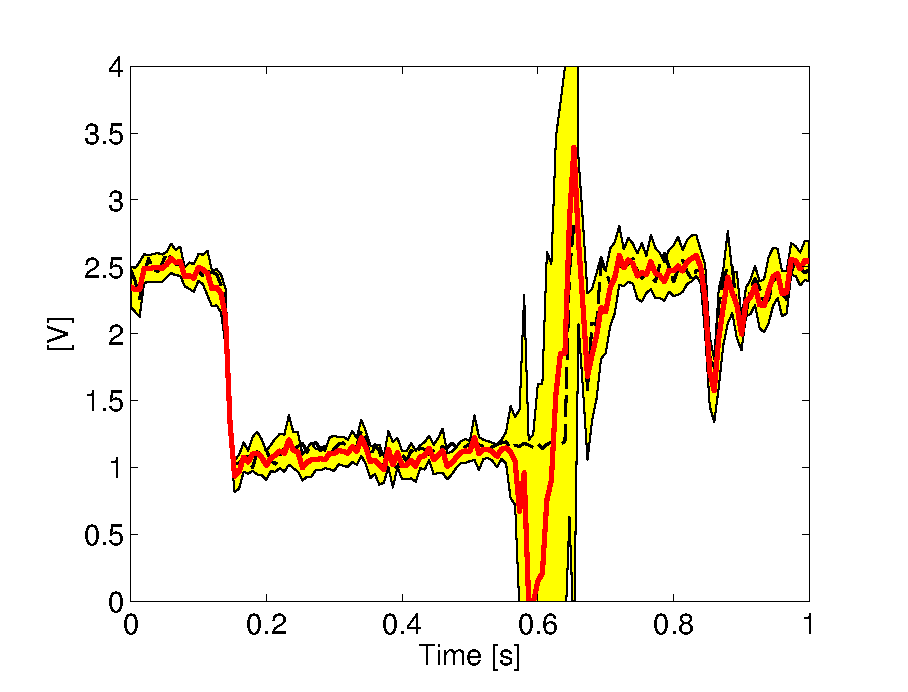
\includegraphics[width=.3\textwidth]{Figures/LLR-LeoIncrMemStep_Foot2}
\label{fig:LLR-LeoIncrMemStep_N2}
}\\
\subfigure[Memory size: $N=6000$ (80 steps)]{
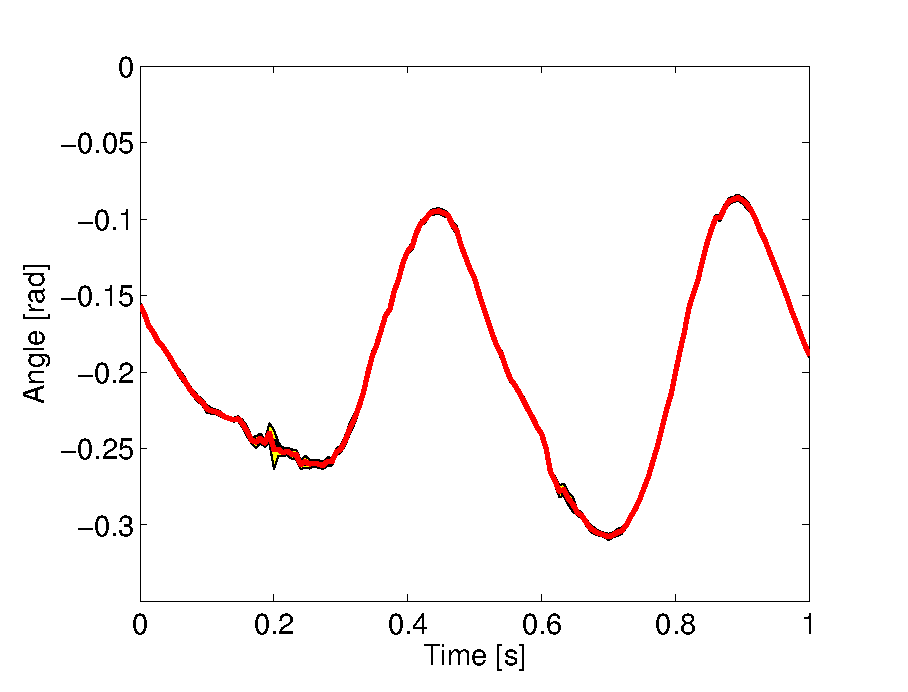
\includegraphics[width=.3\textwidth]{Figures/LLR-LeoIncrMemStep_Torso3}
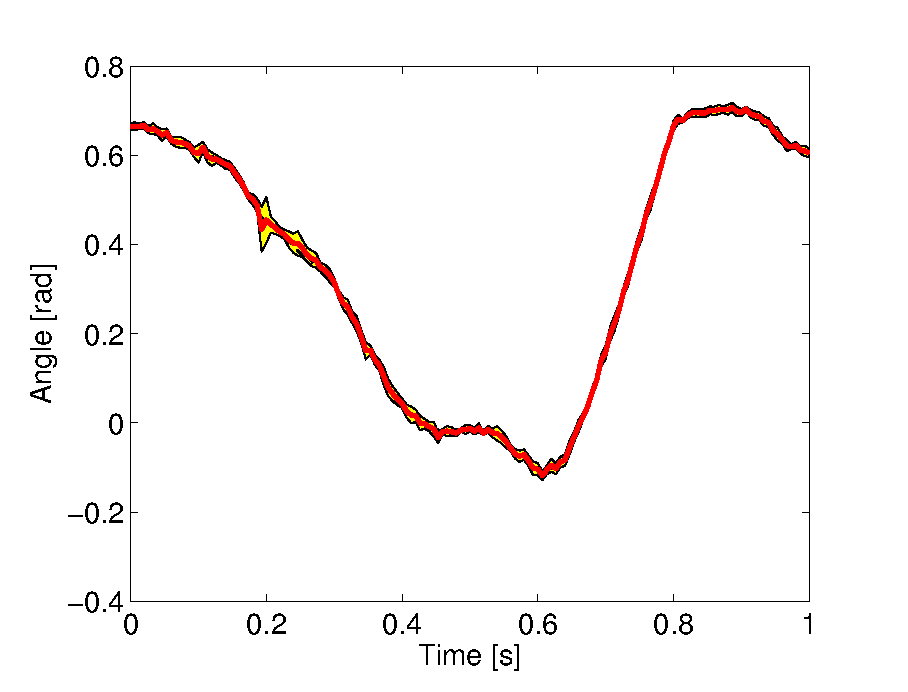
\includegraphics[width=.3\textwidth]{Figures/LLR-LeoIncrMemStep_HipLeft3}
\includegraphics[width=.3\textwidth]{Figures/LLR-LeoIncrMemStep_Foot3}
\label{fig:LLR-LeoIncrMemStep_N3}
} 
\caption[\ac{LLR} estimate of Leo walking for increasing memory size]{Improvement of the \ac{LLR} estimate ($K=40$) of the walking motion of Leo when the memory size increases. The figures show the improvement of the \ac{LLR} estimate for the torso (left), the left hip (middle) and the left foot (right). \subref{fig:LLR-LeoIncrMemStep_N1} is the estimate for a memory of size $N=150$ (roughly 2 steps), \subref{fig:LLR-LeoIncrMemStep_N2} the estimate for $N=1000$ (14 steps) and \subref{fig:LLR-LeoIncrMemStep_N3} for $N=6000$ (80 steps). The figures show the \ac{LLR} estimate (solid red line), the measured value (dashed black line) and the prediction interval (shaded area).}
\label{fig:LLR-LeoIncrMemStep}
\end{figure}

\begin{figure}[htbp]
	\centering
		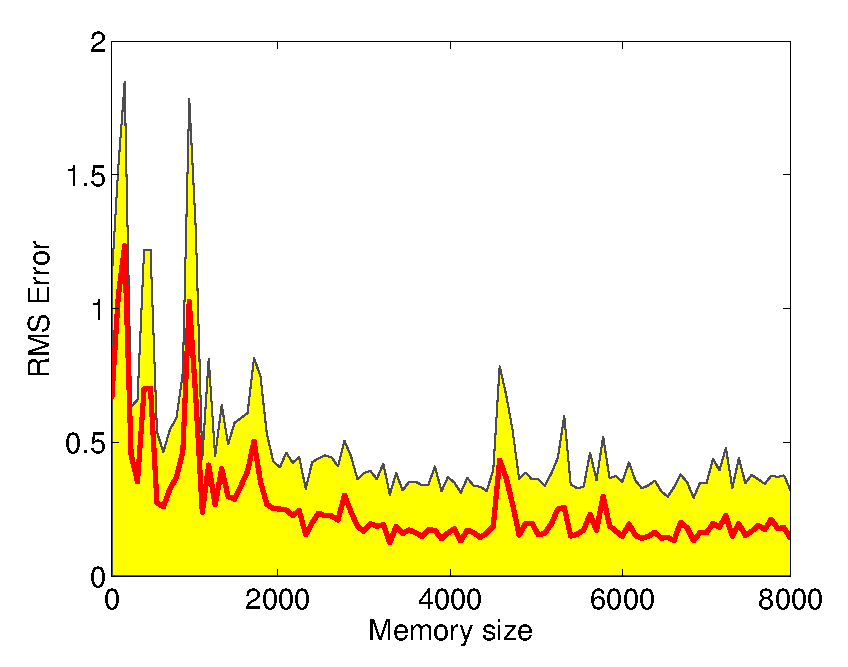
\includegraphics[width=.5\textwidth]{Figures/LLR-LeoIncrMemError}
	\caption[Estimation error for robot Leo for increasing memory size]{\ac{RMS} value of the \ac{LLR} estimation error (solid red line) for the walking motion of Leo for increasing memory size. The shaded area is the \ac{RMS} value of the prediction interval.}
	\label{fig:LLR-LeoIncrMemError}
\end{figure}

%\paragraph{Backwards model} Show that the model can be used in reverse order (using $x_t$ as input and $x_{t-1}$ as output) 






\section{Conclusions}\label{sec:LLR-conclusion}
In this chapter we have introduced \acl{LLR} as method for estimating a model from a set of observed state-transitions. Being a memory-based method, it is easy to implement several results from statistical analysis. Although the number of statistical quantities is vast, we have only described prediction intervals and outlier detection which could be useful in a reinforcement learning setting. In order to decrease the computation time, we introduced a $k$d-tree as a structure to store the samples in the memory. We have shown how the tree structure can be used to search for nearest neighbors more efficiently than a standard sorting approach. 

The capabilities of the \ac{LLR} method were shown in different settings. We used a 1-dimensional nonlinear function to research the possibility to increase the prediction accuracy. We showed that optimizing the number of nearest neighbors locally, can in some cases reduce the estimation error. Also outlier detection was able to identify spikes in the data and resulted in better estimates by neglecting these faulty samples. However, the extra computational effort that is needed to improve the estimate only slightly, makes it not interesting for on-line usage. The prediction interval is a measure for the linearity in the points used in the linear regression and can therefore be used as a rough estimate of the uncertainty in the prediction. 

We applied \ac{LLR} on a two-link manipulator simulation to test its ability to estimate state-transitions. We showed that \ac{LLR} is indeed usable for estimating state-transitions accurately. As expected, increasing the number of samples in the memory, led to an improvement in the estimation accuracy. Furthermore, we showed that fitting a linear model to the set of nearest neighbors (as is done in \ac{LLR}) makes the estimation more accurate compared to memory-based methods that use the average or the nearest neighbor as output.

An important question was whether the \ac{LLR} modeling method still performed well on a complex, noisy system. We answered this question by applying \ac{LLR} on a complex, humanoid robot setup. The \ac{LLR} method proved to be able to model the walking motion of the robot accurately using a relatively small memory of a few thousand samples. One reason that the model is accurate lies in the fact that in all experiments the estimation and validation data are in the same region of state-space. Although this might seem to be an overly ideal situation, this is in fact a reasonable imitation of a real learning process. Not all parts of the state-space are expected to be equally important and we suspect that a perfect model is not needed in all parts, but mainly along trajectories that lead to goal states.

In this chapter, the accuracy of a model was only determined by looking at the response of the model compared to the real system and by inspecting the prediction intervals. The important question whether or not a model is accurate enough to be used in a \ac{RL} setting is deferred to the next chapter where it will be discussed in more detail. 


